\documentclass[aspectratio=169,11pt]{beamer}
% ==========================================================================
%  KSA lecture-slide theme  =  stock beamer "Boadilla"  +  KSA colour theme
%  brand colours sampled from the official KSA symbol mark:
%    Deep Prussian Blue  #2E3192   (지성 - intellect)
%    Golden Gray         #D6CBB1   (감성 - sensibility)
%  Engine: XeLaTeX.  Usage:
%    \documentclass[aspectratio=169,11pt]{beamer}
%    % ==========================================================================
%  KSA lecture-slide theme  =  stock beamer "Boadilla"  +  KSA colour theme
%  brand colours sampled from the official KSA symbol mark:
%    Deep Prussian Blue  #2E3192   (지성 - intellect)
%    Golden Gray         #D6CBB1   (감성 - sensibility)
%  Engine: XeLaTeX.  Usage:
%    \documentclass[aspectratio=169,11pt]{beamer}
%    % ==========================================================================
%  KSA lecture-slide theme  =  stock beamer "Boadilla"  +  KSA colour theme
%  brand colours sampled from the official KSA symbol mark:
%    Deep Prussian Blue  #2E3192   (지성 - intellect)
%    Golden Gray         #D6CBB1   (감성 - sensibility)
%  Engine: XeLaTeX.  Usage:
%    \documentclass[aspectratio=169,11pt]{beamer}
%    \input{../theme/ksa-theme.tex}
% ==========================================================================

\usepackage{fontspec}
\usepackage{amsmath,amssymb}
\usepackage{graphicx}
\graphicspath{{figs/}{../figs/}}
\usepackage{booktabs}
\usepackage{listings}

% ---- fonts (no ctex/xeCJK on this box -> fontspec drives CJK directly) -----
\defaultfontfeatures{Ligatures=TeX}
\setmainfont{Noto Sans CJK KR}
\setsansfont{Noto Sans CJK KR}
\setmonofont{Noto Sans Mono CJK KR}[Scale=0.92]

% ---- base theme: stock Boadilla ------------------------------------------
\usetheme{Boadilla}
\usefonttheme{professionalfonts}
\setbeamertemplate{navigation symbols}{}

% ---- KSA colour theme (recolour the stock theme) --------------------------
\definecolor{ksablue}{HTML}{2E3192}
\definecolor{ksabluedk}{HTML}{20226A}
\definecolor{ksagold}{HTML}{D6CBB1}
\definecolor{ksagolddk}{HTML}{A9976B}
\definecolor{ksared}{HTML}{C0392B}
\definecolor{ksagray}{HTML}{5B5B5B}

\setbeamercolor{structure}{fg=ksablue}
\setbeamercolor{alerted text}{fg=ksared}

\setbeamercolor{palette primary}{fg=white,           bg=ksablue}
\setbeamercolor{palette secondary}{fg=white,         bg=ksablue!85!black}
\setbeamercolor{palette tertiary}{fg=white,          bg=ksabluedk}
\setbeamercolor{titlelike}{fg=ksablue}
\setbeamercolor{frametitle}{fg=ksablue,bg=}
\setbeamercolor{title}{fg=ksablue}
\setbeamercolor{author}{fg=ksagray}
\setbeamercolor{institute}{fg=ksagray}
\setbeamercolor{block title}{fg=white,bg=ksablue}
\setbeamercolor{block body}{fg=black!85,bg=ksablue!6}
\setbeamercolor{item}{fg=ksablue}
\setbeamercolor{section in toc}{fg=black!85}

\setbeamerfont{frametitle}{series=\bfseries}
\setbeamerfont{title}{series=\bfseries}

% ---- footline:  KSA mark | "Made by ..." | n / N   (matches reference) ----
\newcommand{\ksacredit}{Made by Sumin Han \,\textperiodcentered\, suminhan@ksa.hs.kr}
\setbeamertemplate{footline}{%
  \hbox{%
    \begin{beamercolorbox}[wd=.18\paperwidth,ht=2.6ex,dp=1.5ex,leftskip=1.1em]{}%
      \raisebox{-0.35ex}{
\includegraphics[height=2.0ex]{ksa-logo.png}}%
    \end{beamercolorbox}%
    \begin{beamercolorbox}[wd=.64\paperwidth,ht=2.6ex,dp=1.5ex,center]{}%
      {\scriptsize\color{ksagray}\ksacredit}%
    \end{beamercolorbox}%
    \begin{beamercolorbox}[wd=.18\paperwidth,ht=2.6ex,dp=1.5ex,rightskip=1.1em]{}%
      \hfill{\scriptsize\color{ksablue}\insertframenumber\,/\,\inserttotalframenumber}%
    \end{beamercolorbox}%
  }%
  \vskip2pt
}

% ---- section divider: stock \sectionpage, KSA-coloured -------------------
\setbeamertemplate{section page}{%
  \begingroup\centering
    {\color{ksagolddk}\rule{0.16\paperwidth}{1pt}}\par\vskip1.0em
    {\usebeamerfont{title}\color{ksablue}\insertsectionhead\par}\vskip1.0em
    {\color{ksagolddk}\rule{0.16\paperwidth}{1pt}}\par
  \endgroup
}
\AtBeginSection[]{\begin{frame}[plain,noframenumbering]\vfill\sectionpage\vfill\end{frame}}

% ---- code listings ------------------------------------------------------------
\lstdefinestyle{ksa}{%
  basicstyle=\ttfamily\scriptsize,
  keywordstyle=\color{ksablue}\bfseries,
  commentstyle=\color{ksagray}\itshape,
  stringstyle=\color{ksagolddk},
  numberstyle=\tiny\color{ksagray},
  backgroundcolor=\color{ksablue!6},
  frame=leftline, framerule=1.4pt, rulecolor=\color{ksablue},
  xleftmargin=1em, aboveskip=0.8em, belowskip=0.4em,
  showstringspaces=false, breaklines=true, language=Python,
}
\lstset{style=ksa}

% ---- handy macros -----------------------------------------------------------
\newcommand{\kb}[1]{\textbf{\color{ksablue}#1}}   % blue keyword
\newcommand{\kq}[1]{\textbf{\color{ksared}#1}}    % red key-question

% ==========================================================================

\usepackage{fontspec}
\usepackage{amsmath,amssymb}
\usepackage{graphicx}
\graphicspath{{figs/}{../figs/}}
\usepackage{booktabs}
\usepackage{listings}

% ---- fonts (no ctex/xeCJK on this box -> fontspec drives CJK directly) -----
\defaultfontfeatures{Ligatures=TeX}
\setmainfont{Noto Sans CJK KR}
\setsansfont{Noto Sans CJK KR}
\setmonofont{Noto Sans Mono CJK KR}[Scale=0.92]

% ---- base theme: stock Boadilla ------------------------------------------
\usetheme{Boadilla}
\usefonttheme{professionalfonts}
\setbeamertemplate{navigation symbols}{}

% ---- KSA colour theme (recolour the stock theme) --------------------------
\definecolor{ksablue}{HTML}{2E3192}
\definecolor{ksabluedk}{HTML}{20226A}
\definecolor{ksagold}{HTML}{D6CBB1}
\definecolor{ksagolddk}{HTML}{A9976B}
\definecolor{ksared}{HTML}{C0392B}
\definecolor{ksagray}{HTML}{5B5B5B}

\setbeamercolor{structure}{fg=ksablue}
\setbeamercolor{alerted text}{fg=ksared}

\setbeamercolor{palette primary}{fg=white,           bg=ksablue}
\setbeamercolor{palette secondary}{fg=white,         bg=ksablue!85!black}
\setbeamercolor{palette tertiary}{fg=white,          bg=ksabluedk}
\setbeamercolor{titlelike}{fg=ksablue}
\setbeamercolor{frametitle}{fg=ksablue,bg=}
\setbeamercolor{title}{fg=ksablue}
\setbeamercolor{author}{fg=ksagray}
\setbeamercolor{institute}{fg=ksagray}
\setbeamercolor{block title}{fg=white,bg=ksablue}
\setbeamercolor{block body}{fg=black!85,bg=ksablue!6}
\setbeamercolor{item}{fg=ksablue}
\setbeamercolor{section in toc}{fg=black!85}

\setbeamerfont{frametitle}{series=\bfseries}
\setbeamerfont{title}{series=\bfseries}

% ---- footline:  KSA mark | "Made by ..." | n / N   (matches reference) ----
\newcommand{\ksacredit}{Made by Sumin Han \,\textperiodcentered\, suminhan@ksa.hs.kr}
\setbeamertemplate{footline}{%
  \hbox{%
    \begin{beamercolorbox}[wd=.18\paperwidth,ht=2.6ex,dp=1.5ex,leftskip=1.1em]{}%
      \raisebox{-0.35ex}{
\includegraphics[height=2.0ex]{ksa-logo.png}}%
    \end{beamercolorbox}%
    \begin{beamercolorbox}[wd=.64\paperwidth,ht=2.6ex,dp=1.5ex,center]{}%
      {\scriptsize\color{ksagray}\ksacredit}%
    \end{beamercolorbox}%
    \begin{beamercolorbox}[wd=.18\paperwidth,ht=2.6ex,dp=1.5ex,rightskip=1.1em]{}%
      \hfill{\scriptsize\color{ksablue}\insertframenumber\,/\,\inserttotalframenumber}%
    \end{beamercolorbox}%
  }%
  \vskip2pt
}

% ---- section divider: stock \sectionpage, KSA-coloured -------------------
\setbeamertemplate{section page}{%
  \begingroup\centering
    {\color{ksagolddk}\rule{0.16\paperwidth}{1pt}}\par\vskip1.0em
    {\usebeamerfont{title}\color{ksablue}\insertsectionhead\par}\vskip1.0em
    {\color{ksagolddk}\rule{0.16\paperwidth}{1pt}}\par
  \endgroup
}
\AtBeginSection[]{\begin{frame}[plain,noframenumbering]\vfill\sectionpage\vfill\end{frame}}

% ---- code listings ------------------------------------------------------------
\lstdefinestyle{ksa}{%
  basicstyle=\ttfamily\scriptsize,
  keywordstyle=\color{ksablue}\bfseries,
  commentstyle=\color{ksagray}\itshape,
  stringstyle=\color{ksagolddk},
  numberstyle=\tiny\color{ksagray},
  backgroundcolor=\color{ksablue!6},
  frame=leftline, framerule=1.4pt, rulecolor=\color{ksablue},
  xleftmargin=1em, aboveskip=0.8em, belowskip=0.4em,
  showstringspaces=false, breaklines=true, language=Python,
}
\lstset{style=ksa}

% ---- handy macros -----------------------------------------------------------
\newcommand{\kb}[1]{\textbf{\color{ksablue}#1}}   % blue keyword
\newcommand{\kq}[1]{\textbf{\color{ksared}#1}}    % red key-question

% ==========================================================================

\usepackage{fontspec}
\usepackage{amsmath,amssymb}
\usepackage{graphicx}
\graphicspath{{figs/}{../figs/}}
\usepackage{booktabs}
\usepackage{listings}

% ---- fonts (no ctex/xeCJK on this box -> fontspec drives CJK directly) -----
\defaultfontfeatures{Ligatures=TeX}
\setmainfont{Noto Sans CJK KR}
\setsansfont{Noto Sans CJK KR}
\setmonofont{Noto Sans Mono CJK KR}[Scale=0.92]

% ---- base theme: stock Boadilla ------------------------------------------
\usetheme{Boadilla}
\usefonttheme{professionalfonts}
\setbeamertemplate{navigation symbols}{}

% ---- KSA colour theme (recolour the stock theme) --------------------------
\definecolor{ksablue}{HTML}{2E3192}
\definecolor{ksabluedk}{HTML}{20226A}
\definecolor{ksagold}{HTML}{D6CBB1}
\definecolor{ksagolddk}{HTML}{A9976B}
\definecolor{ksared}{HTML}{C0392B}
\definecolor{ksagray}{HTML}{5B5B5B}

\setbeamercolor{structure}{fg=ksablue}
\setbeamercolor{alerted text}{fg=ksared}

\setbeamercolor{palette primary}{fg=white,           bg=ksablue}
\setbeamercolor{palette secondary}{fg=white,         bg=ksablue!85!black}
\setbeamercolor{palette tertiary}{fg=white,          bg=ksabluedk}
\setbeamercolor{titlelike}{fg=ksablue}
\setbeamercolor{frametitle}{fg=ksablue,bg=}
\setbeamercolor{title}{fg=ksablue}
\setbeamercolor{author}{fg=ksagray}
\setbeamercolor{institute}{fg=ksagray}
\setbeamercolor{block title}{fg=white,bg=ksablue}
\setbeamercolor{block body}{fg=black!85,bg=ksablue!6}
\setbeamercolor{item}{fg=ksablue}
\setbeamercolor{section in toc}{fg=black!85}

\setbeamerfont{frametitle}{series=\bfseries}
\setbeamerfont{title}{series=\bfseries}

% ---- footline:  KSA mark | "Made by ..." | n / N   (matches reference) ----
\newcommand{\ksacredit}{Made by Sumin Han \,\textperiodcentered\, suminhan@ksa.hs.kr}
\setbeamertemplate{footline}{%
  \hbox{%
    \begin{beamercolorbox}[wd=.18\paperwidth,ht=2.6ex,dp=1.5ex,leftskip=1.1em]{}%
      \raisebox{-0.35ex}{
\includegraphics[height=2.0ex]{ksa-logo.png}}%
    \end{beamercolorbox}%
    \begin{beamercolorbox}[wd=.64\paperwidth,ht=2.6ex,dp=1.5ex,center]{}%
      {\scriptsize\color{ksagray}\ksacredit}%
    \end{beamercolorbox}%
    \begin{beamercolorbox}[wd=.18\paperwidth,ht=2.6ex,dp=1.5ex,rightskip=1.1em]{}%
      \hfill{\scriptsize\color{ksablue}\insertframenumber\,/\,\inserttotalframenumber}%
    \end{beamercolorbox}%
  }%
  \vskip2pt
}

% ---- section divider: stock \sectionpage, KSA-coloured -------------------
\setbeamertemplate{section page}{%
  \begingroup\centering
    {\color{ksagolddk}\rule{0.16\paperwidth}{1pt}}\par\vskip1.0em
    {\usebeamerfont{title}\color{ksablue}\insertsectionhead\par}\vskip1.0em
    {\color{ksagolddk}\rule{0.16\paperwidth}{1pt}}\par
  \endgroup
}
\AtBeginSection[]{\begin{frame}[plain,noframenumbering]\vfill\sectionpage\vfill\end{frame}}

% ---- code listings ------------------------------------------------------------
\lstdefinestyle{ksa}{%
  basicstyle=\ttfamily\scriptsize,
  keywordstyle=\color{ksablue}\bfseries,
  commentstyle=\color{ksagray}\itshape,
  stringstyle=\color{ksagolddk},
  numberstyle=\tiny\color{ksagray},
  backgroundcolor=\color{ksablue!6},
  frame=leftline, framerule=1.4pt, rulecolor=\color{ksablue},
  xleftmargin=1em, aboveskip=0.8em, belowskip=0.4em,
  showstringspaces=false, breaklines=true, language=Python,
}
\lstset{style=ksa}

% ---- handy macros -----------------------------------------------------------
\newcommand{\kb}[1]{\textbf{\color{ksablue}#1}}   % blue keyword
\newcommand{\kq}[1]{\textbf{\color{ksared}#1}}    % red key-question


\title{고급 시뮬레이션: MuJoCo와 Isaac Sim}
\subtitle{MuJoCo 정밀 물리 실습 · GPU 병렬의 원리 · 정밀도$\times$속도 도구 선택 · 자율주행 시뮬레이션}
\author{Machine Learning 2 \,\textperiodcentered\, 14주차}
\institute{한국과학영재학교 (KSA)}
\date{Chapter 14}

\begin{document}

% ===== title =====
\begin{frame}[plain,noframenumbering]
  \titlepage
\end{frame}

% ===== roadmap of this week =====
\begin{frame}{이번 주차 개요}
  \textbf{이 챕터를 마치면}
  \begin{enumerate}
    \item Gymnasium 래퍼 없이 \kb{MuJoCo} XML로 로봇을 직접 정의하고,
      무작위 정책과 PD 제어 정책으로 D항(속도 피드백)이 왜 필요한지
      궤적으로 설명할 수 있다.
    \item ``시간 방향 의존성'' 때문에 한 환경은 병렬화할 수 없고,
      병렬의 대상은 \textbf{환경(초깃값이 다른 복제본)}임을 실측 숫자로
      설명할 수 있다.
    \item GPU 가속의 핵심(모든 상태를 한 텐서에 담아 커널 한 번)을
      ML1 Ch.\,10.1의 CNN과 비교해 설명하고, numpy로 1,000개 진자를
      동시에 시뮬레이션할 수 있다.
    \item 정밀도 축$\times$속도 축 실측 steps/s로 네 도구(Gymnasium\,·
      PyBullet\,· MuJoCo\,· Isaac Sim) 고르는 \textbf{30초 결정 절차}를
      스스로 적용할 수 있다.
    \item 자율주행의 Onboard/Offboard 루프가 policy iteration/Dyna
      구조와 같은 모양인 이유와 \kb{SceneDiffuser}의 역할을 개념
      수준으로 설명할 수 있다.
  \end{enumerate}
  \vskip0.5em
  \small
  \begin{itemize}
    \item \kb{14.1} XML 진자 정의 · 무작위 vs PD 제어 · 30줄 래퍼 · LCP 접촉
    \item \kb{14.2} CPU의 ``하나씩'' 한계 · 커널 한 번 · 1,000 진자 실측 76배
    \item \kb{14.3} 네 도구 한 표 · 정밀도/속도 두 축 · 30초 결정 절차
    \item \kb{14.4} Waymo Onboard/Offboard 루프 · policy iteration · diffusion 시나리오
  \end{itemize}
  \vskip0.4em
  \kq{같은 RL 알고리즘 위에 시뮬레이터를 교체하면, 무엇이 바뀌고
  무엇이 그대로 남는가?}
\end{frame}

\section{14.1 MuJoCo와 정책 학습 실습}

\begin{frame}{장난감 환경에서 실체 물리엔진으로}
  \begin{itemize}
    \item Ch.\,13의 Gymnasium 기본 환경: 물리를 \textbf{간단한 근사식}으로
      계산 --- 빠르지만 접촉·마찰은 거칠게 흉내만 냄
    \item 실전 로봇 연구: 접촉(contact), 마찰 등 중요한 물리 현상은
      \textbf{훨씬 정교한 물리엔진}이 필요
  \end{itemize}
  \vskip0.6em
  \small
  \begin{tabular}{@{}ll@{}}
    \toprule
    도구 & 특징 \\
    \midrule
    \kb{MuJoCo} (2012, Todorov) & CPU에서 도는 \textbf{정밀} 물리엔진 ---
      접촉·마찰을 LCP로 매 스텝 해결 \\
    \kb{Isaac Sim} (NVIDIA) & GPU로 \textbf{수천 개} 시뮬레이션을
      동시에 --- 렌더링 포함 \\
    \bottomrule
  \end{tabular}
  \vskip0.7em
  \begin{block}{이번 장이 줄곧 묻는 질문}
    \kq{같은 강화학습 알고리즘 위에 시뮬레이터를 교체했을 때,
    무엇이 바뀌고 무엇이 그대로 남는가?}
  \end{block}
  정밀하고 빠른 물리는 어디까지 필요한가, 그 비용을 누가 지불하는가
  --- 실측 숫자까지 붙여 답한다.
\end{frame}

\begin{frame}{이 장의 위치: 알고리즘은 그대로, 시뮬레이터만 올린다}
  \begin{itemize}
    \item Ch.\,13의 전제: ``\textbf{시뮬레이터 안에서 먼저 익히고,
      이후에 실물로 옮긴다}''
      (PPO로 Reacher 학습 · 평가 프로토콜 · reality gap 대응)
    \item 이번 장: \textbf{알고리즘은 그대로 두고}, 시뮬레이터 자체를
      실전 연구 수준으로 올리는 장
  \end{itemize}
  \vskip0.6em
  \begin{block}{직접 확인해볼 사실}
    같은 \texttt{env.step()} 위에 \textbf{물리엔진만 바꾸면 된다}
    --- 14.1에서 30줄 래퍼로 시연, 14.2에서는 ``GPU로만 옮긴다''로
    그 차이를 실측한다.
  \end{block}
  \vskip0.5em
  \begin{itemize}
    \item 다음 장(Ch.\,15)은 물리 모델이 \textbf{주어지지 않는} 문제 ---
      모델이 \textit{학습될 대상}이 되는 경우 (MCTS\,· World Models)
    \item 시뮬레이터가 주는 경험인지, 배운 모델이 주는 경험인지에 따라
      \textbf{경험을 모으는 방식}이 달라진다 --- 그 계산부터 짚어둔다
  \end{itemize}
\end{frame}

\begin{frame}[fragile]{MuJoCo: XML로 모델, mj\_step으로 시뮬레이션}
  MuJoCo(Multi-Joint dynamics with Contact)는 관절·접촉·마찰을
  물리적으로 정확하게 계산하는 엔진 --- 2021년 무료 공개 후 로봇 RL
  연구의 사실상 표준. 모델은 \textbf{XML}로 정의한다:
\begin{lstlisting}
import mujoco
xml = """
<mujoco>
  <worldbody>
    <light name="top" pos="0 0 1"/>
    <geom type="plane" size="1 1 0.1"/>
    <body pos="0 0 1">
      <joint type="free"/>
      <geom type="sphere" size="0.1" rgba="1 0 0 1"/>
    </body>
  </worldbody>
</mujoco>
"""
model = mujoco.MjModel.from_xml_string(xml)
data = mujoco.MjData(model)
for step in range(5):
    mujoco.mj_step(model, data)  # 물리 법칙에 따라 한 스텝 전진
print("5스텝 후 공의 높이:", round(data.qpos[2], 4))
\end{lstlisting}
\end{frame}

\begin{frame}{자유낙하로 검산: 한 스텝 $\approx$ 0.002초}
  \begin{itemize}
    \item \texttt{free} 관절: 위치 $q_{pos}$ 7개 성분, 속도 $q_{vel}$ 6개 ---
      공 하나만 떠 있어도 상태가 이 정도
    \item 방향을 4차원 \kb{쿼터니언}으로: 유러 각은 \textbf{짐벌 락}
      기이점에서 계산이 깨지지만, 쿼터니언은 안 깨진다
    \item 5스텝: 1.0000 $\to$ 0.9994\,m (아직은 아주 조금)
  \end{itemize}
  \vskip0.6em
  \begin{block}{검산: 50스텝($\approx$0.1초)}
    자유낙하 공식 $h = 1 - \tfrac12 gt^2$ 의 예측은 \textbf{0.951\,m} ---
    실제 시뮬레이션 값 \textbf{0.95\,m}으로 거의 정확히 일치.
    즉 \texttt{mj\_step} 한 번 = 물리 시간 약 \textbf{0.002초}.
  \end{block}
  \vskip0.5em
  \begin{itemize}
    \item 같은 API(\texttt{MjModel}\,/\,\texttt{MjData}\,/\,\texttt{mj\_step})로
      다리가 여러 개인 로봇, 로봇팔, 인간형까지 표현
    \item Gymnasium의 \texttt{HalfCheetah}\,·\,\texttt{Ant}\,·\,\texttt{Humanoid}
      --- Ch.\,13.2의 \texttt{Reacher-v5}\,·\,\texttt{Ant-v5}도 이 엔진 위에 있다
  \end{itemize}
\end{frame}

\begin{frame}{환경이 바뀌어도 알고리즘은 그대로 (선언)}
  \begin{itemize}
    \item Ch.\,9--13에서 배운 DQN·PPO: 환경이 CartPole이든
      MuJoCo 기반 로봇이든 \textbf{바뀌지 않는다}
    \item \texttt{env.step()} 인터페이스만 지키면, 물리엔진이
      훨씬 정교해져도 \textbf{알고리즘 쪽 코드는 그대로}
  \end{itemize}
  \vskip0.6em
  \begin{block}{이 절에서 할 일}
    선언을 멈추고 \textbf{시연}으로 바꾼다 --- Gymnasium 래퍼 없이
    MuJoCo API를 직접 써서 진자 하나를 정의하고 제어한다.
  \end{block}
  \vskip0.5em
  \begin{columns}[T]
    \begin{column}{0.5\textwidth}
      \kb{관절(joint)} \texttt{hinge}: 한 축만 회전
    \end{column}
    \begin{column}{0.5\textwidth}
      \kb{액추에이터(actuator)} \texttt{motor}: 그 관절에
      토크를 가하는 모터
    \end{column}
  \end{columns}
\end{frame}

\begin{frame}[fragile]{실습: XML로 진자 + PD 제어 정책}
\begin{lstlisting}
import mujoco
import numpy as np
xml = """
<mujoco>
  <option gravity="0 0 -9.81"/>
  <worldbody>
    <body pos="0 0 1">
      <joint name="hinge" type="hinge" axis="0 1 0"
             damping="0.1"/>
      <geom type="capsule" fromto="0 0 0  0 0 -0.5"
            size="0.02" mass="1"/>
    </body>
  </worldbody>
  <actuator>
    <motor joint="hinge" gear="1" ctrlrange="-5 5"/>
  </actuator>
</mujoco>
"""
model = mujoco.MjModel.from_xml_string(xml)
data = mujoco.MjData(model)
data.qpos[0] = 3.0        # 목표(0)에서 멀리 떨어뜨려 시작
mujoco.mj_forward(model, data)

# PD 제어 정책: 각도가 클수록, 각속도가 클수록 반대 방향으로 토크
for _ in range(200):
    theta, thetadot = data.qpos[0], data.qvel[0]
    data.ctrl[0] = np.clip(-3.0*theta - 0.5*thetadot, -5, 5)
    mujoco.mj_step(model, data)
\end{lstlisting}
\end{frame}

\begin{frame}{진자 모델의 요소들}
  \begin{itemize}
    \item $q_{pos}$: 1개 --- 힌지 각도 $\theta$ \quad
      $q_{vel}$: 1개 --- 각속도 $\dot\theta$
    \item $\theta=0$: 막대가 아래로 수직인 \textbf{자연 휴식 상태}
      (목표)
    \item \texttt{damping}=$0.1$: 관절 자체의 마찰 --- 속도에 비례해
      반대 방향 힘을 \textbf{자동}으로 가함
  \end{itemize}
  \vskip0.5em
  \begin{tabular}{@{}ll@{}}
    \toprule
    항목 & 의미 \\
    \midrule
    \texttt{capsule fromto} & 축(0,0,0)에서 끝(0,0,-0.5)까지 0.5\,m 막대 \\
    \texttt{ctrl} & \textbf{우리가} 매 스텝 직접 지정하는 토크 \\
    실제 힘 & \texttt{ctrl} + 마찰력 합산 \\
    \bottomrule
  \end{tabular}
  \vskip0.6em
  \begin{block}{\kb{PD(Proportional--Derivative, 비례-미분) 제어}}
    토크 $= -3\,\theta - 0.5\,\dot\theta$
    --- \textbf{P항}: 각도만큼 반대 힘 / \textbf{D항}: 각속도만큼
    ``브레이크''
  \end{block}
\end{frame}

\begin{frame}{200스텝 비교: 무작위 vs PD}
  200스텝 실행 검증 (seed 0):
  \small
  \begin{tabular}{@{}ll@{}}
    \toprule
    정책 & 결과 \\
    \midrule
    무작위 정책 & 평균 $|\theta| = 2.97$ (초기 3.0에서 거의 안 줄어듦) \\
    PD 제어 정책 & 평균 $|\theta| = 1.69$, \textbf{최종} $\theta = -0.065$ \\
    \bottomrule
  \end{tabular}
  \vskip0.7em
  \begin{columns}[T]
    \begin{column}{0.52\textwidth}
      \centering
      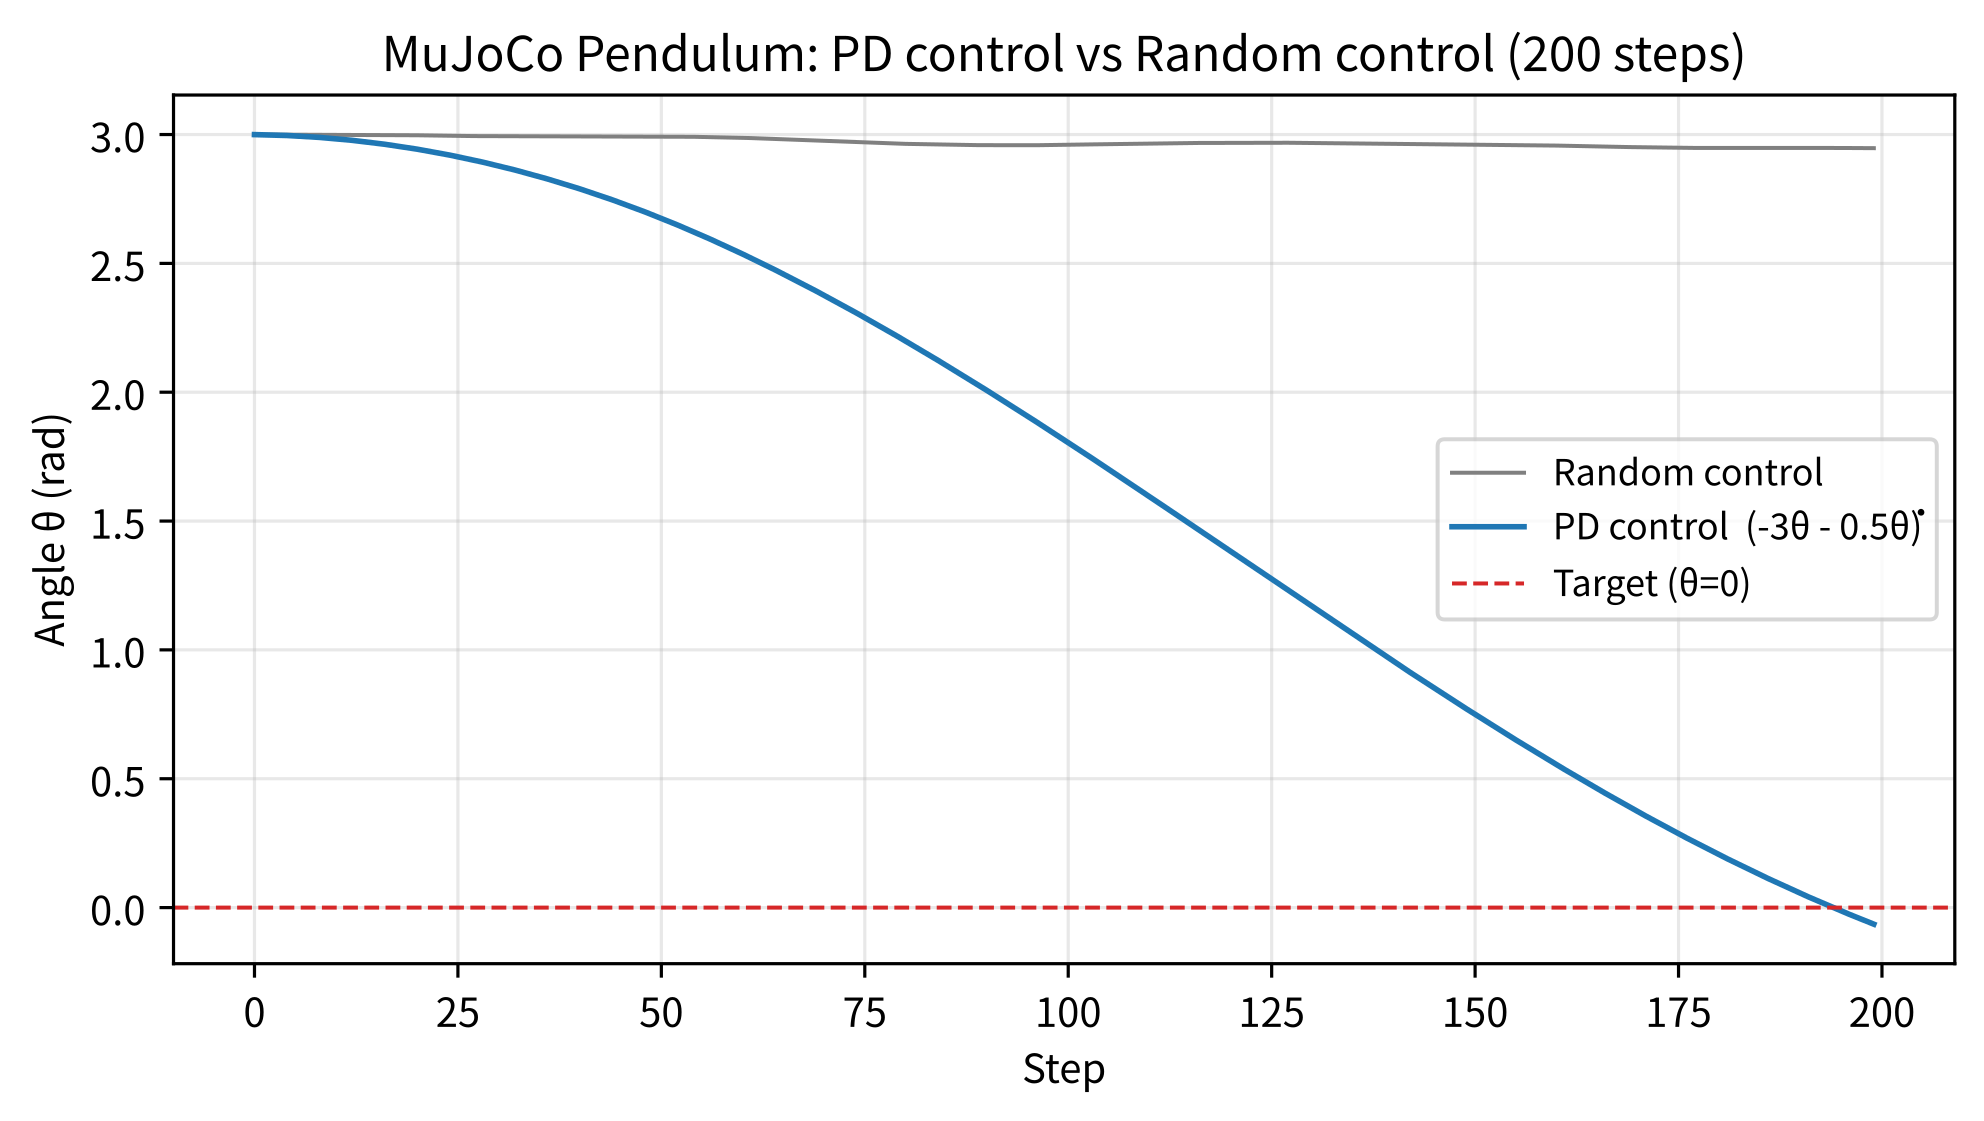
\includegraphics[width=\linewidth]{ch14_1_pendulum_pd_vs_random.png}
    \end{column}
    \begin{column}{0.44\textwidth}
      {\footnotesize \textbf{파란 실선(PD)}: 큰 진폭으로 흔들리다가
      진폭이 줄며 거의 0(목표)에 안착.
      \textbf{회색 선(무작위)}: $\pm\pi$ 안에서 이리저리 떠돌다
      처음 위치(약 3.0) 근처에 그대로 머문다.
      $\theta$ 단위: 라디안.}
    \end{column}
  \end{columns}
  \vskip0.3em
  \begin{itemize}
    \item Ch.\,13.2에서 이미 본 패턴 --- 이번엔 \textbf{래퍼 없이}
      \texttt{MjModel}\,/\,\texttt{MjData}\,/\,\texttt{mj\_step}을 직접 다룸
  \end{itemize}
\end{frame}

\begin{frame}{``평균 1.69인데 최종 -0.065'' --- 모순인가}
  \begin{itemize}
    \item 모순이 아니다 --- 두 정책이 \textbf{어디에 있느냐}가 아니라
      \textbf{어떻게 움직이느냐}를 보여주는 차이
    \item PD는 \kb{감쇠 진동}: 진폭이 갈수록 작아지는 진동
  \end{itemize}
  \vskip0.5em
  \begin{block}{숫자가 다른 이유}
    200스텝 \textbf{중간}에는 여전히 큰 각도에서 자주 지남
    $\Rightarrow$ 평균이 1.69로 높다. 200스텝 \textbf{끝}에는 이미
    중심(0) 근처 $\Rightarrow$ 최종값 $-0.065$.
    완전한 안착($|\theta|<0.1$ \textbf{그리고} $|\dot\theta|<0.1$)은
    약 \textbf{680스텝}쯤에야 온다.
  \end{block}
  \vskip0.5em
  \begin{itemize}
    \item 무작위 정책은 평균도 최종값도 2.9 --- ``처음과 거의
      같은 자리''에 있다는 점이 핵심
  \end{itemize}
  {\footnotesize 실전: Gymnasium이 아직 환경을 만들어 두지 않은
  커스텀 로봇을 RL로 제어하려면, 정확히 이 수준(XML로 모델 정의 +
  \texttt{ctrl} 배열에 행동)에서 Gymnasium 환경 클래스를 직접 작성한다.}
\end{frame}

\begin{frame}{자주 하는 실수: D항을 빼거나 부호를 뒤집으면}
  ``PD가 마법처럼 보인다'' --- 그 마법의 대부분은 \textbf{D항}
  $(-0.5\,\dot\theta)$에서 온다. 이득만 바꿔 200스텝 실행 검증:
  \small
  \begin{tabular}{@{}p{4.2cm}p{3.6cm}p{5.6cm}@{}}
    \toprule
    정책 (토크) & 200스텝 후 $|\theta|$ & 결과 \\
    \midrule
    \textbf{완전한 PD} $\;-3\theta - 0.5\dot\theta\;$ & 0.065 &
      목표(0)에 접근 \\
    \textbf{P만} $\;-3\theta\;$ & 1.31 (각속도까지 11.5!) &
      크게 진동만 함 \\
    \textbf{너무 약한 PD} $\;-1\theta - 0.2\dot\theta\;$ & 0.69 &
      거의 못 줌 \\
    \textbf{부호 오류} $\;+3\theta - 0.5\dot\theta\;$ & 7.62 &
      발산(목표와 반대) \\
    \textbf{제어 없음} (0) & 2.60 & 처음 그대로 \\
    \bottomrule
  \end{tabular}
\end{frame}

\begin{frame}{왜 P만으론 ``위험한 고속 진동''인가}
  \begin{itemize}
    \item P항(``각도가 크면 반대 방향으로 힘'')만으론: 막대가
      \textbf{중심을 지날 때마다 관성으로 과속} $\Rightarrow$ 한쪽 끝까지
      쏘아올리고, 다시 반대쪽으로
    \item 마찰(\texttt{damping})이 아주 적어 에너지가 거의 안 줄므로
      $|\theta|\approx1.3$, 각속도 11.5에 갇힘
    \item \kb{D항}: 각속도에 비례해 ``지금은 빨리 가니까 브레이크''
      힘을 덧붙여 \textbf{진동을 죽여}준다
  \end{itemize}
  \vskip0.6em
  \begin{itemize}
    \item 부호 오류($+3\theta$): ``각도가 크면 더 크게 \textbf{같은
      방향}으로'' $\Rightarrow$ 시스템에 \textbf{에너지 주입} $\Rightarrow$
      발산
    \item $\theta=0$이 \textbf{안정 균형점}(아래로 처진 상태)인지
      \textbf{불안정 균형점}(위에서 균형)인지 틀리면,
      아무리 잘 학습해도 안착하지 않는다
  \end{itemize}
\end{frame}

\begin{frame}{확인: D항 없이 학습은 될까?}
  \begin{block}{RL과의 직결}
    정책 그래디언트로 ``어떤 토크가 좋은가''를 배우려면, 좋은 정책
    (D항 포함)과 나쁜 정책(P만)의 \textbf{리턴이 확실하게 달라야} 한다.
  \end{block}
  \vskip0.5em
  \begin{itemize}
    \item P만으로 200스텝을 못 넘기거나 발산 $\Rightarrow$ 보상 신호가
      ``이 정책은 처참하다'' $\Rightarrow$ \textbf{학습이 오히려 쉬워짐}
    \item \textbf{약하지만 P만} 같은 ``아까운 실패''(0.69) $\Rightarrow$
      보상 차이가 작아 \textbf{신호가 희미}해진다
  \end{itemize}
  \vskip0.6em
  \begin{block}{원리}
    물리적으로 안정하지 않은 정책은, 강화학습이 \textbf{수학적으로}
    배우기 전에 물리 시뮬레이션이 먼저 \textbf{안정적으로} 살아야
    하는 이유다.
  \end{block}
\end{frame}

\begin{frame}{물리 시뮬레이터를 Gymnasium ``환경''으로 감싸기}
  \begin{itemize}
    \item Ch.\,9--13의 알고리즘(DQN, PPO)을 이 MuJoCo 진자에
      그대로 달아본다
    \item 필요한 것은 \textbf{딱 하나} --- MuJoCo를
      \texttt{(s, a, r, done)}을 돌려주는 \texttt{reset()}\,/\,
      \texttt{step()} 인터페이스로 \textbf{감싸는} 작은 클래스
  \end{itemize}
  \vskip0.5em
  \begin{columns}[T]
    \begin{column}{0.5\textwidth}
      \kb{\texttt{reset()}}
      \begin{itemize}
        \item $q_{pos}$ 초기화
        \item (상태, 정보) 반환
      \end{itemize}
    \end{column}
    \begin{column}{0.5\textwidth}
      \kb{\texttt{step(action)}}
      \begin{itemize}
        \item \texttt{ctrl}에 행동 넣고 \texttt{mj\_step}
        \item (다음 상태, 보상, 종료 여부) 반환
      \end{itemize}
    \end{column}
  \end{columns}
  \vskip0.5em
  {\footnotesize 이 30줄 클래스는 \texttt{Reacher-v5}\,·\,\texttt{Ant-v5}가
  내부에서 하는 일의 \textbf{미니판}이다.}
\end{frame}

\begin{frame}[fragile]{30줄 래퍼: MuJoCoPendulum}
\begin{lstlisting}
class MuJoCoPendulum:
    """raw MuJoCo 진자를 Gymnasium 스타일 (s, a, r, done) 환경으로 감싼다."""
    def __init__(self, seed=0):
        self.model = mujoco.MjModel.from_xml_string(xml)  # 위의 xml
        self.data = mujoco.MjData(self.model)
        self.rng = np.random.default_rng(seed)
        self.max_steps = 200

    def reset(self, seed=None):
        if seed is not None:
            self.rng = np.random.default_rng(seed)
        self.data.qpos[0] = 3.0          # 목표에서 먼 각도
        self.data.qvel[0] = 0.0
        mujoco.mj_forward(self.model, self.data)
        self.t = 0
        return np.array([self.data.qpos[0], self.data.qvel[0]]), {}

    def step(self, action):
        self.data.ctrl[0] = float(np.clip(action, -5, 5))  # 토크 한도
        mujoco.mj_step(self.model, self.data)
        th = self.data.qpos[0]
        reward = -th * th                 # 0에 가까울수록 보상 큼
        self.t += 1
        done = self.t >= self.max_steps
        s = np.array([self.data.qpos[0], self.data.qvel[0]])
        return s, float(reward), bool(done), False, {}
\end{lstlisting}
\end{frame}

\begin{frame}{핵심 메시지: 시연된 사실}
  이 \texttt{MuJoCoPendulum}에 PD 정책을 그대로 걸어 200스텝:
  \small
  \begin{tabular}{@{}ll@{}}
    \toprule
    정책 & 결과 \\
    \midrule
    PD & 최종 $(\theta, \dot\theta) = (-0.065, -6.26)$,
      누적 보상 $-777$ \\
    무작위 & 평균 $|\theta| = 2.97$ \\
    \bottomrule
  \end{tabular}
  \vskip0.5em
  $\Rightarrow$ 바로 위에서 \texttt{mj\_step}을 직접 돌린 결과와
  \textbf{완전히 같다}.
  \vskip0.7em
  \begin{block}{이번 절의 핵심}
    ``환경이 CartPole이든 MuJoCo 로봇이든 \textbf{알고리즘은
    바뀌지 않는다}'' --- 이번엔 선언이 아니라 \textbf{30줄 래퍼로
    시연된 사실}. \texttt{gym.make("Pendulum-v1")}을
    \texttt{MuJoCoPendulum()}로 바꾸는 \textbf{한 줄}만 고치면
    DQN·PPO 코드가 그대로 동작한다.
  \end{block}
\end{frame}

\begin{frame}{왜 MuJoCo가 ``정밀''한가: LCP 접촉}
  \begin{itemize}
    \item ``정밀''은 속도나 모델 크기가 아니다 --- 핵심은
      \kb{접촉(contact)}을 푸는 방식
    \item 공이 바닥에 \textbf{닿는 순간}은 단순 미분방정식이 아니다:
  \end{itemize}
  \vskip0.4em
  \begin{block}{두 조건이 ``동시에''}
    \textbf{비침투}(non-penetration): 겹쳐 들어가면 안 되지만
    --- \textbf{비음}(non-negativity): 겹치지 않을 땐 힘 필요 없음
    $\Rightarrow$ 수학적으로 \kb{선형 보완 문제(LCP, Linear
    Complementarity Problem)}라는 특별한 형태의 최적화
  \end{block}
  \vskip0.5em
  \begin{itemize}
    \item MuJoCo는 이 LCP를 \textbf{매 스텝}에서 안정적으로 풀어낸다
  \end{itemize}
\end{frame}

\begin{frame}{LCP를 매 스텝 푸는 것의 값}
  \begin{enumerate}
    \item 공이 바닥에 부딪혀 튕기거나 멈추는 행위가 \textbf{계산이
      깨지지 않고}(폭주/NaN 없이) 자연스러워짐
    \item 다리 로봇의 발이 바닥에 붙었다 떨어지기를 반복하는
      \textbf{걸음} 같은 복잡한 접촉도 같은 식으로 처리
  \end{enumerate}
  \vskip0.6em
  \begin{block}{반대편: ``단단한 막대'' 방식}
    접촉을 강제 제약으로만 푸는 엔진: \textbf{여러 접촉이 동시에}
    일어나는 경우(예: 네 다리로 서 있는 로봇) 제약이 서로
    충돌해 \textbf{계산이 불안정}해지기 쉬움
  \end{block}
  \vskip0.5em
  \begin{itemize}
    \item 14.2\,·\,14.3에서 ``다리 로봇을 학습시킬 땐 왜 정밀 물리엔진이
      필요한가''를 논할 때, 그 필요성의 \textbf{뿌리}가 바로 이
      LCP 접촉 솔버에 있다
  \end{itemize}
\end{frame}

\begin{frame}{역사: 모델 기반 제어의 물리엔진}
  \begin{itemize}
    \item 2012, Todorov: \textit{``MuJoCo: A physics engine for
      model-based control''} (IROS 2012) --- 이름은 \textbf{Mu}lti-
      \textbf{J}oint dynamics with \textbf{C}ontact
    \item 처음부터 ``로봇 재현''이 아니라 \kb{모델 기반 제어}
      (시스템 모델을 알고, 그 모델을 최적 제어에 넣는 방식)의
      \textbf{재현성과 속도}를 위해 설계
    \item 접촉을 LCP로 푸는 것 역시 이 \textbf{최적화 관점의
      자연스러운 결과}
  \end{itemize}
  \vskip0.6em
  \begin{itemize}
    \item 2021: 무료 오픈소스화 $\Rightarrow$ GPU 병렬 시뮬레이터
      (14.2 Isaac Sim)가 없어도 \textbf{CPU에서 정밀 로봇 물리}가
      가능
    \item OpenAI \texttt{gym}에서 DeepMind 로봇 연구까지
      \textbf{사실상 표준 물리엔진}
  \end{itemize}
  \vskip0.4em
  {\footnotesize 이번 절의 XML로 모델 정의 + \texttt{ctrl}에 값 넣기
  = 이 ``모델 기반''의 ``모델''을 \textbf{손으로 만져보는} 것.}
\end{frame}

\begin{frame}{자주 묻는 질문 (14.1)}
  \small
  \begin{itemize}
    \item \textbf{Q. \texttt{qpos}\,·\,\texttt{qvel}\,·\,\texttt{ctrl}은?}
      $q_{pos}$ = 위치 자유도(관절 각도, 물체 위치),
      $q_{vel}$ = 그 시간 미분(각속도, 속도) --- MDP 상태
      $\mathcal{S}$가 바로 이 $(q_{pos}, q_{vel})$의 조합.
      \texttt{ctrl} = 액추에이터에 가하는 제어 입력(토크) ---
      MDP의 행동 $\mathcal{A}$에 해당.
    \item \textbf{Q. 왜 굳이 MuJoCo API를 직접 쓰나?}
      기존 환경(Reacher, Ant)은 Gymnasium 래퍼가 편리하지만,
      ``세상에 없는 새로운 로봇''을 시뮬레이션하려면 XML로 직접
      정의해야 한다 --- Gymnasium의 MuJoCo 환경도 내부적으로
      정확히 이 API를 감싸고 있을 뿐이다.
  \end{itemize}
\end{frame}

\begin{frame}{자주 묻는 질문 (14.1): PPO를 그대로 돌리면?}
  \begin{itemize}
    \item \textbf{Q. 직접 만든 환경에 Ch.\,13.2 PPO를 그대로?}
      \texttt{reset()}\,/\,\texttt{step()} 시그니처를 지키면
      \texttt{env} 인자로 \texttt{MuJoCoPendulum()}을 받기만 하면 된다.
      \textbf{두 가지 실전 차이}:
  \end{itemize}
  \vskip0.4em
  \begin{enumerate}
    \item \kb{보상의 스케일} --- PPO의 GAE·어드밴티지 정규화는
      보상 범위에 민감. 진자의 ``$-$각도$^2$'' 보상이 CartPole의
      ``$+1$/스텝''보다 절대값이 크면 \textbf{정규화 파라미터를
      다시 맞춰}야 한다
    \item \kb{시드 결정성} --- Gymnasium은
      \texttt{env.reset(seed=...)}로 결정적 시드를 보장, 직접 만든
      클래스는 \texttt{reset}에서 시드를
      \texttt{np.random.default\_rng}에 넘겨줘야
      ``같은 시드 $\to$ 같은 궤적''이 성립
      (코드에서 \texttt{self.rng}가 그 역할)
  \end{enumerate}
  \vskip0.5em
  {\footnotesize 확인 문제 예시: \texttt{done}을
  \texttt{abs(th) < 0.1}로 바꾸면 PPO의 리턴 $G_t$ 길이에 어떻게
  영향을 주는가? (``에피소드가 목표 달성 시 조기 종료'' + 성공/실패를
  보상과 연결하는 방식)
  }
\end{frame}

\section{14.2 NVIDIA Isaac Sim과 GPU 가속의 원리}

\begin{frame}{Isaac Sim: GPU로 수천 개를 동시에}
  \begin{itemize}
    \item \kb{Isaac Sim} (NVIDIA): Omniverse 플랫폼 위의 로봇
      시뮬레이션 환경 --- 물리 계산 \textbf{자체}를 GPU에서
      병렬로 수행
    \item 같은 로봇 환경을 CPU에서 하나씩 순차로 도는 대신,
      \textbf{수천 개의 복제본}을 GPU 위에서 동시에
    \item 사실적인 렌더링(카메라 센서 시뮬레이션)까지 ---
      ``\textbf{픽셀을 보고 판단하는}'' 로봇 정책 학습에도 널리 사용
  \end{itemize}
  \vskip0.6em
  \begin{block}{단, 이번 학기 실습에서는 시연 영상으로만}
    최소 사양: \textbf{RTX 4080 (16GB VRAM)}급 이상, \textbf{RT 코어}
    필요 --- RT 코어가 없는 A100\,·\,H100류 데이터센터 GPU는
    \textbf{미지원}. 학교의 GPU가 바로 H100/H200 계열이라 실습에서
    직접 돌릴 수 없다.
  \end{block}
\end{frame}

\begin{frame}{그렇다면 오늘 50분은 무엇을 하는가}
  Isaac Sim을 못 돌리더라도, ``Isaac Sim이 빠르다''고 말할 때
  \textbf{그 빠름이 수학적으로 어디서 오는지}는 CPU 위에서,
  numpy 한 줄로 직접 재볼 수 있다.
  \vskip0.6em
  \small
  \begin{tabular}{@{}cl@{}}
    \toprule
    단계 & 내용 \\
    \midrule
    (1) & CPU가 환경 스텝을 \textbf{``하나씩''}만 돌릴 수 있는
      이유를 \textbf{숫자}로 확인 \\
    (2) & Isaac Sim이 그 한계를 어떻게 우회하는지
      (모든 상태를 한 배열에 담아 \textbf{커널을 한 번} 호출)
      구조도로 보고 \\
    (3) & 그 아이디어를 14.1의 진자를 \textbf{1,000개 복제}해
      numpy로 직접 시뮬레이션 · 실험 \\
    \bottomrule
  \end{tabular}
  \vskip0.5em
  \begin{itemize}
    \item 실측 머신: 학교 서버 CPU (2026-08, 워밍업 200스텝 제외)
  \end{itemize}
\end{frame}

\begin{frame}{먼저 숫자로: 같은 CPU에서 40배}
  \small
  \begin{tabular}{@{}llr@{}}
    \toprule
    환경 & 물리 수준 & 초당 스텝 수 \\
    \midrule
    CartPole-v1 (Gymnasium 기본) & 단순 근사 & 약 242,000 \\
    Pendulum (MuJoCo, 14.1의 진자) & 정밀(단일 관절) & 약 246,000 \\
    Ant-v5 (MuJoCo, 사족보행) & 정밀(복잡한 접촉) & 약 5,900 \\
    \bottomrule
  \end{tabular}
  \vskip0.7em
  \begin{itemize}
    \item \textbf{같은 CPU}에서도 환경에 따라 약 \textbf{40배} 차이
      --- ``CPU''라는 틀이 속도를 정하는 게 아니라,
      \textbf{어떤 물리를 계산하느냐}가 정한다
      (14.1의 LCP 접촉이 매 스텝 푸는 계산이 그 차이의 정체)
    \item 10억 스텝이면: CartPole
      $10^9/2.4\times10^5 \approx 4{,}100$초 $\approx$
      \textbf{약 1.2시간}
    \item 같은 10억 스텝을 Ant(5,900 steps/s)로:
      $\approx 1.7\times10^5$초 $\approx$ \textbf{약 2일}
  \end{itemize}
\end{frame}

\begin{frame}{왜 속도를 2배·100배·수천 배로 늘리기가 이렇게 어려운가}
  \begin{itemize}
    \item 현대 CPU: 8$\sim$64개 코어 --- 코어가 16개면
      \textbf{독립 작업} 16개까지 동시 가능
    \item 그런데 ``환경 하나를 스텝시키기''는 \textbf{독립 작업이
      아니다}
  \end{itemize}
  \vskip0.5em
  \begin{block}{\kb{시간 방향 의존성}}
    한 환경의 $t$스텝은 같은 환경의 $t-1$스텝 결과가 나와야만
    계산이 시작된다.
  \end{block}
  \vskip0.5em
  \begin{itemize}
    \item 이 의존성을 깨는 방법은 ``같은 환경의 시간을 잘게
      나누는 것''이 \textbf{아니다}
    \item $\Rightarrow$ \textbf{서로 다른 환경}(=초깃값이 다른
      복제본)을 코어마다 하나씩 맡기는 것
    \item 예: 16코어 CPU로 Ant 16개를 병렬 $\Rightarrow$
      Ant 16개 환경 스텝을 동시 계산 --- 이것이 ``CPU 병렬''의
      \textbf{전부}
  \end{itemize}
\end{frame}

\begin{frame}{그 ``전부''가 문제: CPU 병렬의 상한선}
  \begin{itemize}
    \item 16코어 $\times$ 5,900 steps/s $\approx$ \textbf{약 9.4만
      steps/s}가 실질적 상한 (코어당 메모리 대역폭, 스레드 간
      동기화 오버헤드를 감안하면 실제로는 그보다 낮음)
    \item Ant 10억 스텝: 2일 $\to$ \textbf{약 12시간}으로 줄어드는
      것뿐 --- ``이틀을 기다리자''에서 ``하루를 포기하자''
  \end{itemize}
  \vskip0.6em
  \begin{block}{결론}
    수천 개 복제본이 필요한 \textbf{대규모 보행 연구}(14.3:
    10억+ 스텝)에서는 이 상한선이 \textbf{결정적}이다.
    바로 이 벽을 부수러 온 것이 \kb{GPU}이고, 그 벽을 실제로 부수고
    그대로 시뮬레이터로 상품화한 것이 \kb{Isaac Sim}이다.
  \end{block}
\end{frame}

\begin{frame}{GPU 가속 시뮬레이션의 원리: CNN의 구조}
  \begin{itemize}
    \item CPU 기반 시뮬레이터(MuJoCo, Gymnasium 기본): 한 번에
      \textbf{환경 하나}를 스텝 --- 경험을 더 모으려면 더 많은 시간
    \item GPU 가속 시뮬레이터: 물리 계산 \textbf{자체}를 대규모
      병렬 연산으로 다시 설계
  \end{itemize}
  \vskip0.5em
  \begin{block}{ML1 Ch.\,10.1의 CNN 아이디어}
    ``같은 연산을 위치마다 반복한다'' --- 이번엔
    \textbf{``같은 물리 스텝을 로봇 복제본마다 반복한다''}.
    수천 개 환경을 GPU 코어에 흩뿌려 동시 계산.
  \end{block}
  \vskip0.5em
  \begin{itemize}
    \item 결과: 초당 모을 수 있는 (상태, 행동, 보상) 경험의 양이
      CPU 대비 \textbf{수십$\sim$수백 배}까지
    \item Ch.\,9의 \textbf{경험재현 버퍼}가 순식간에 채워지는 셈
  \end{itemize}
\end{frame}

\begin{frame}{데이터가 GPU 위에서 어떻게 배치되는가}
  \begin{columns}[T]
    \begin{column}{0.56\textwidth}
      \centering
      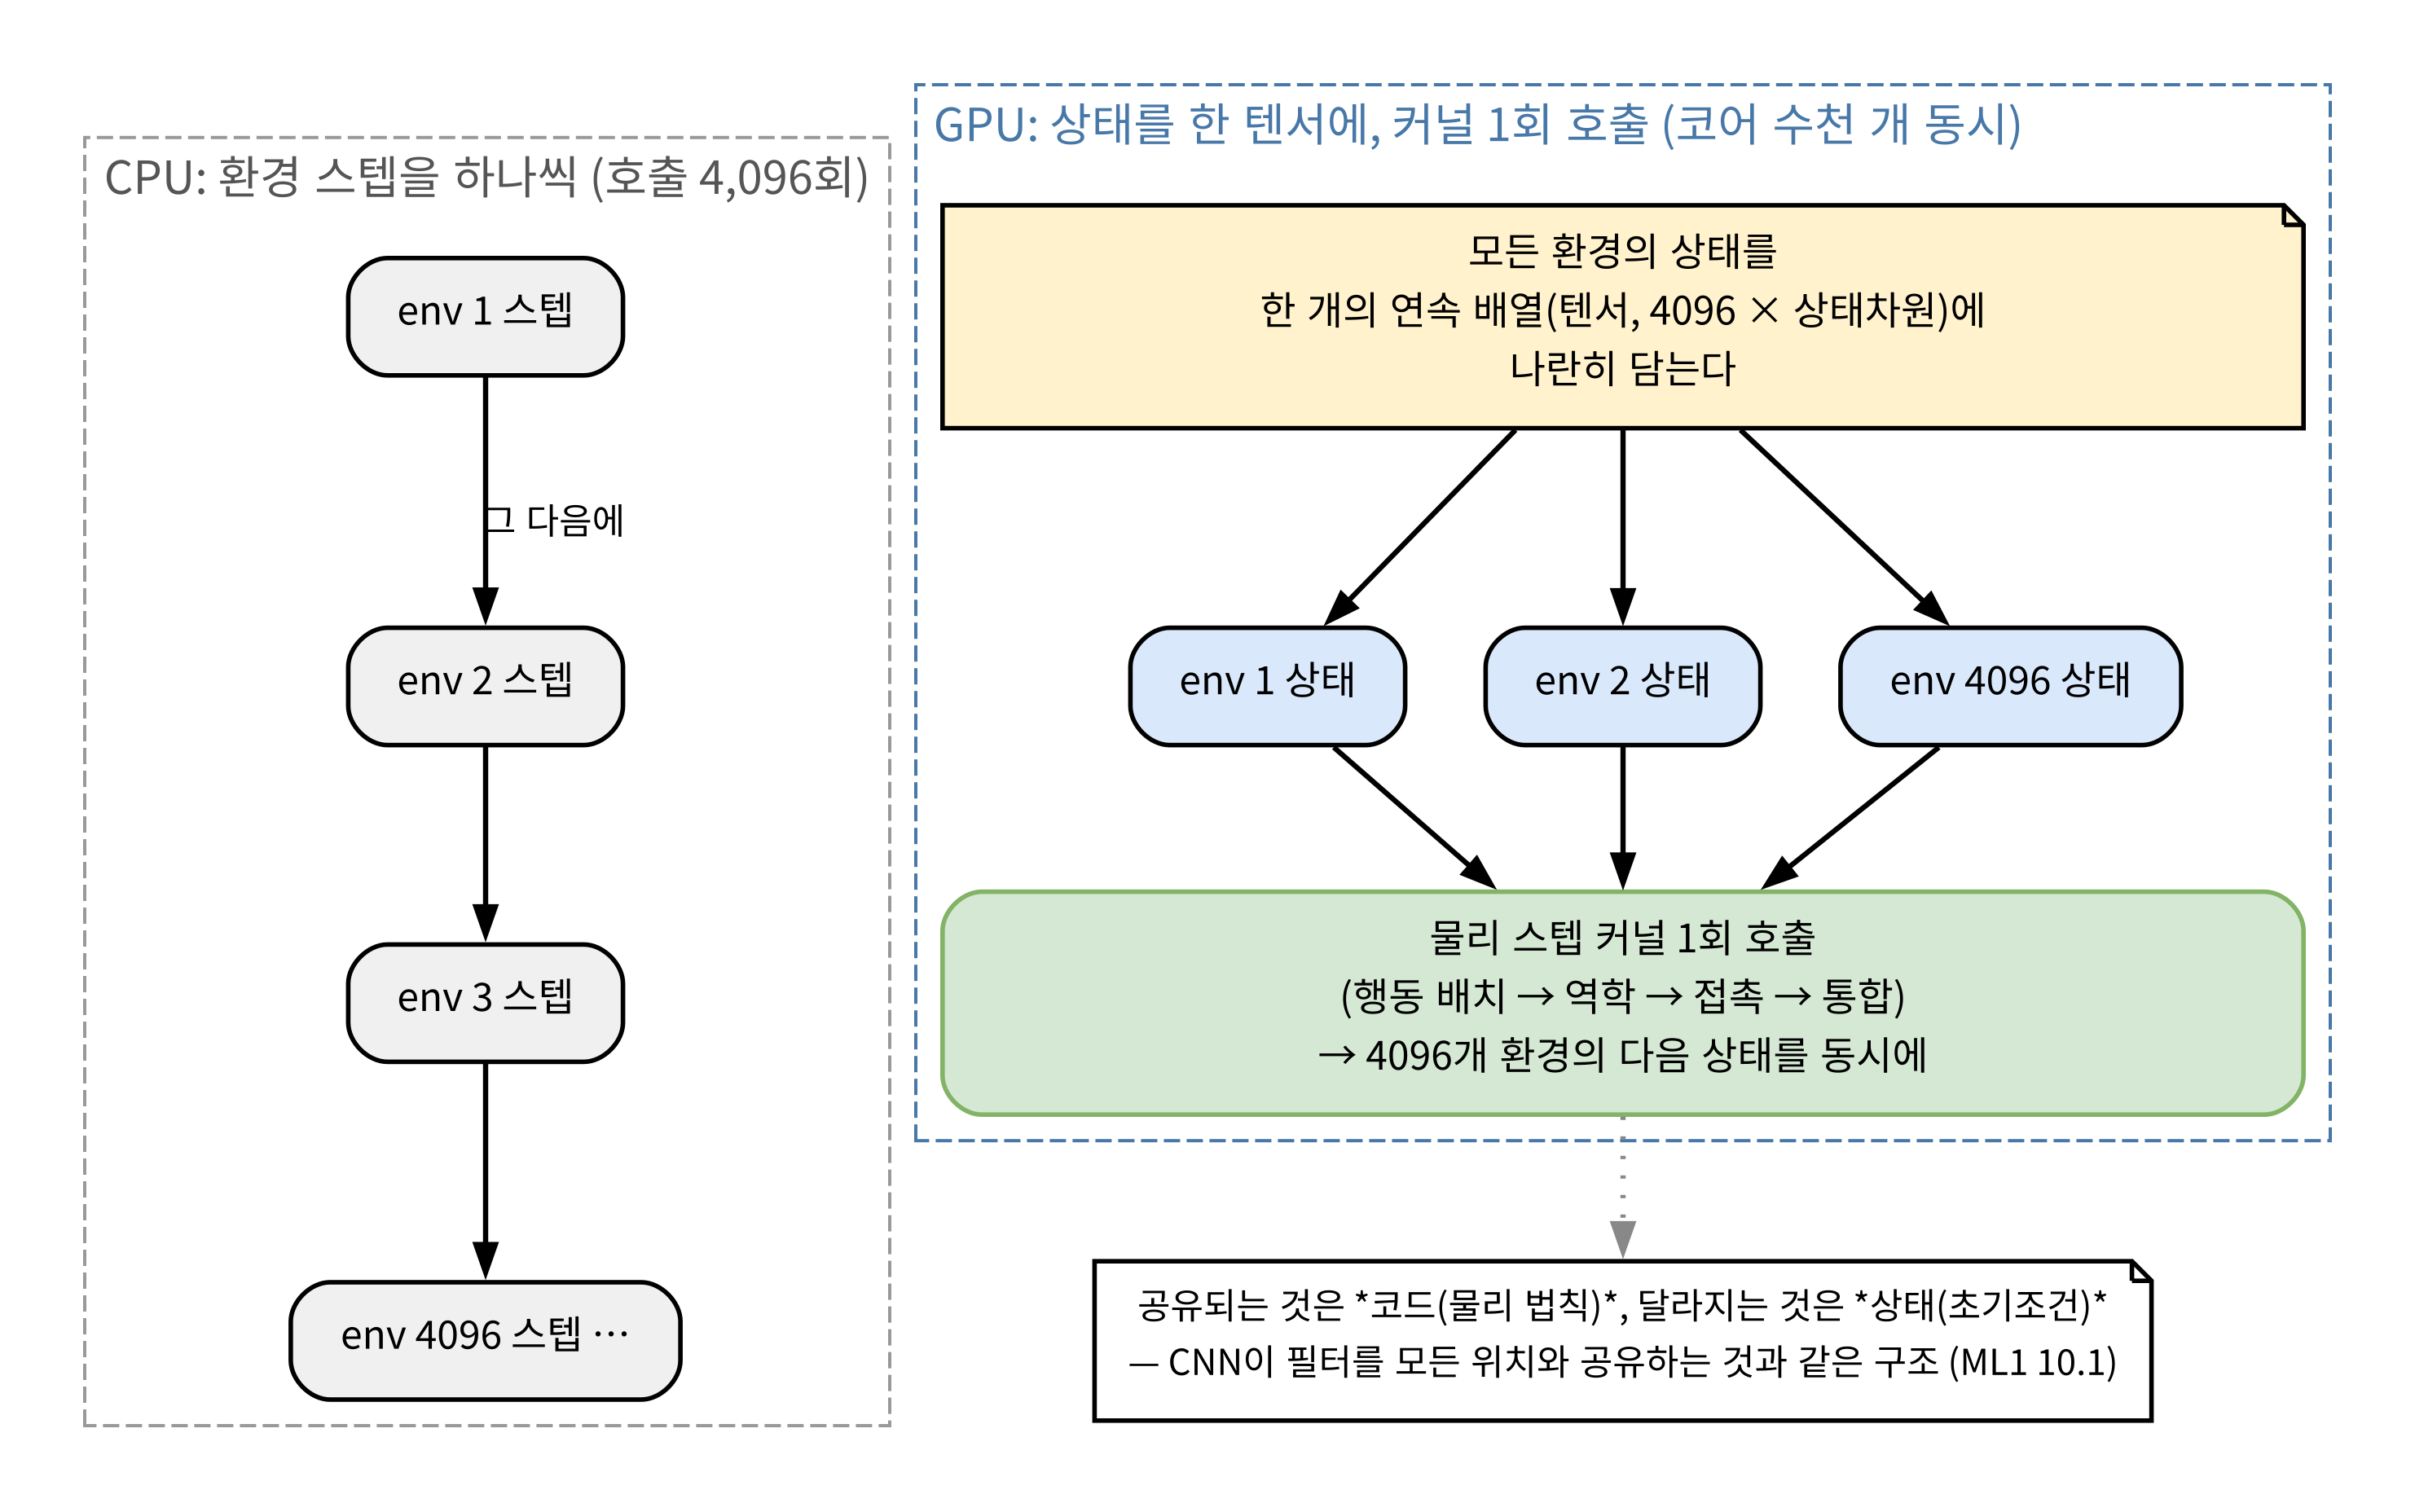
\includegraphics[width=\linewidth]{ch14_2_batch_step_v2.png}
    \end{column}
    \begin{column}{0.40\textwidth}
      {\footnotesize CPU: 환경 스텝을 \textbf{하나씩} 순서대로
      (C1$\to$C2$\to$C3$\to$\ldots). GPU: 4096개 환경의 상태를
      \textbf{한 개의 연속 텐서 배열}에 나란히 담아
      \textbf{물리 스텝 커널 1회 호출}로 4096개 환경의 다음
      상태를 동시 계산.}
    \end{column}
  \end{columns}
  \vskip0.4em
  \begin{itemize}
    \item 그림의 핵심: ``\textbf{모든 환경의 상태를 한 개의 연속
      배열(텐서)에 나란히 담는다}''
    \item GPU가 빠른 이유: ``코어가 많아서''가 아니라,
      \textbf{코어 개수와 데이터가 나란히 배열된 길이가 일치하기
      때문}
  \end{itemize}
\end{frame}

\begin{frame}{커널 한 번의 의미}
  \begin{itemize}
    \item NVIDIA GPU: 수천$\sim$수만 개의 가벼운 코어(CUDA 코어) ---
      모두 \textbf{같은 연산을 나란히 놓인 데이터 요소마다} 수행
     하도록 설계
    \item ``4,096개 환경의 상태''를 하나의 큰 텐서
      $(4096 \times \text{상태차원})$로 모으면:
  \end{itemize}
  \vskip0.5em
  \begin{block}{``커널 한 번''}
    물리 스텝을 계산하는 \kb{커널(kernel) 함수를 한 번만} 호출하면
    수천 개의 코어가 \textbf{각자 자신의 환경}의 물리 스텝을
    동시에 처리. 함수를 4,096번 \textbf{호출하는 게} 아니라,
    \textbf{한 번의 함수 호출 안의 연산이 수천 개로 나뉜다}
    --- 이것이 CPU 순차 호출과의 근본적 차이.
  \end{block}
\end{frame}

\begin{frame}{CNN의 병렬 vs Isaac Sim의 병렬}
  \small
  \begin{tabular}{@{}p{2.6cm}p{5.4cm}p{6.0cm}@{}}
    \toprule
     & CNN의 병렬 (ML1 10.1) & Isaac Sim의 병렬 \\
    \midrule
    반복되는 단위 & 같은 \textbf{필터}(파라미터)를 위치마다
      적용 & 같은 \textbf{물리 스텝}(코드)을 복제본마다 적용 \\
    공유되는 것 & 파라미터 (무게) & 프로그램 (물리 법칙, 코드) \\
    달라지는 것 & 입력 픽셀 (위치마다 다름) & 상태
      (초기조건이 다른 복제본) \\
    병렬의 방향 & 공간(픽셀 위치) & 시간 대신 \textbf{환경}
      (독립 실행 실체) \\
    \bottomrule
  \end{tabular}
  \vskip0.7em
  \begin{block}{공통 뼈대}
    ``\textbf{한 번 작성된 연산을, 나란히 놓인 서로 다른 데이터
    요소에 동시에 적용한다}.''
    CNN은 한 입력 안에서 \textbf{공간적으로} 병렬, Isaac Sim은
    한 물리 법칙 안에 \textbf{환경 단위로} 병렬.
  \end{block}
\end{frame}

\begin{frame}{``복제되는 것은 초깃값''}
  \begin{itemize}
    \item 그래서: CNN이 배운 ``가중치''가 \textbf{필터} 자체인
      반면, Isaac Sim에서 \textbf{복제되는 것은 ``초깃값''}
    \item 수천 개의 진자가 \textbf{같은 물리 법칙}(같은 코드)을
      따르되, $\theta_0$만 다르다
  \end{itemize}
  \vskip0.5em
  \begin{columns}[T]
    \begin{column}{0.48\textwidth}
      \kb{CNN}
      \begin{itemize}
        \item 공유: \textbf{파라미터(필터)}
        \item 변하는: 입력 픽셀
      \end{itemize}
    \end{column}
    \begin{column}{0.48\textwidth}
      \kb{Isaac Sim}
      \begin{itemize}
        \item 공유: \textbf{프로그램(물리 법칙, 코드)}
        \item 변하는: 상태(초기조건)
      \end{itemize}
    \end{column}
  \end{columns}
  \vskip0.6em
  {\footnotesize 이 구분이 다음 실습(1,000개 진자를 $\theta_0$만
  다르게 시작)의 \textbf{설계}에 그대로 쓰인다.}
\end{frame}

\begin{frame}{커널 한 번: 한 스텝이 지나면 (4단계)}
  Isaac Sim 계열 GPU 물리엔진(Warp 기반, MuJoCo-XLA의 CUDA 경로와
  같은 원리)의 한 스텝 순서:
  \small
  \begin{tabular}{@{}cl@{}}
    \toprule
    단계 & 내용 \\
    \midrule
    1. \kb{행동 배치} & 4,096개 환경 각자의 행동 $a_i$를 텐서
      $A \in \mathbb{R}^{4096 \times d_a}$로 수집 \\
    2. \kb{역학 커널} & 모든 복제본의 미분방정식(관성, 중력,
      PD/모터 법칙)을 \textbf{한 번의 커널 호출}로 계산
      --- CUDA 코어가 수천 개 나뉘어 동시 실행되는 곳 \\
    3. \kb{접촉 커널} & 복제본마다 ``무엇이 무엇과 닿는가''를
      \textbf{동시에} 검사 (4,096개 진자가 각각 바닥에 닿았는지
      동시 질문) \\
    4. \kb{통합} & 2$\sim$3의 결과를 모든 복제본에 동시 적용해
      다음 상태 $q_{t+1}$ 산출 \\
    \bottomrule
  \end{tabular}
\end{frame}

\begin{frame}{호출 횟수가 ``4,096$\times$4''에서 ``4''로}
  \begin{itemize}
    \item CPU로 \textbf{순차}: 4,096 $\times$ (4단계)만큼의
      \textbf{연속된 호출}
    \item GPU: 4단계 $\times$ \textbf{1회의 호출}
  \end{itemize}
  \vskip0.5em
  \begin{block}{``수천 배''의 정수적 기원}
    \textbf{호출 횟수(순차성)}가 ``$4{,}096 \times 4$''에서
    ``$4$''로 줄어드는 것. 코어가 4,096개이든 16,384개이든,
    \textbf{호출 한 번 안의 연산이 데이터 길이만큼 나뉜다}는
    구조가 동일하다.
  \end{block}
  \vskip0.5em
  \begin{itemize}
    \item CPU 버전(MuJoCo \texttt{mj\_step})과의 구조적 차이:
      ``환경 $i$에 \texttt{ctrl} 하나''인 인자가, GPU 버전에서는
      \textbf{배열 전체}가 함수 인자가 됨
  \end{itemize}
\end{frame}

\begin{frame}{오버헤드 문제: 왜 ``커널 한 번''이 큰 차이인가}
  \begin{itemize}
    \item CPU: 함수 호출과 결과 수령에 드는 시간(호출 오버헤드,
      캐시 미스, 브랜치 예측 실패)은 \textbf{호출 한 번마다}
      발생
    \item 4,096번 호출 $\Rightarrow$ 4,096번 그 오버헤드를
      \textbf{치른다}
  \end{itemize}
  \vskip0.5em
  \begin{block}{GPU의 구조}
    커널 발기 오버헤드는 \textbf{일단}만 치르고, 그 안에서
    수천 개 코어가 \textbf{동일한 명령}을 나란히 놓인 데이터에
    동시 수행(\kb{SIMT, single-instruction multiple-thread})
    $\Rightarrow$ 오버헤드가 \textbf{데이터 길이와 무관하게
    상수로 묶여} 버린다.
  \end{block}
  \vskip0.5em
  \begin{itemize}
    \item \kb{아몰달의 법칙(Amdahl's Law)}과 연결하면, GPU 병렬의
      ``몇 배까지 빨라질 수 있는가''의 \textbf{이론적 상한}이
      왜 존재하는지 볼 수 있다 (아래 확인)
  \end{itemize}
\end{frame}

\begin{frame}{확인: Amdahl의 법칙}
  파이프라인을 (a) 환경 스텝(병렬화 가능, 비율 $p$)과 (b)
  정책 업데이트 + 동기화(병렬화 불가, 비율 $1-p$)로 나눌 때,
  $N$코어 병렬화 후의 전체 가속은
  \[
    \frac{1}{(1-p) + p/N}
  \]
  \begin{itemize}
    \item $N \to \infty$ 해도 가속은 $\dfrac{1}{1-p}$에 수렴
      --- \textbf{순차 부분이 10\%}($p=0.9$)면, 코어가 무한이어도
      \textbf{최대 10배}에 그침
    \item $p=0.99$ $\Rightarrow$ 100배, $p=0.999$ $\Rightarrow$
      1,000배
  \end{itemize}
  \vskip0.5em
  \begin{block}{Isaac Sim의 엔지니어링}
    ``환경 스텝 $\times$수천''을 달성하려면 $p$가 \textbf{0.999
    이상}. 실제로: 환경 스텝을 \textbf{VRAM 안에서 순환}(호스트
    $\to$ VRAM 왕복 최소화) + 정책 업데이트를 환경 스텝 사이에
    \textbf{삽입(overlap)} $\Rightarrow$ $1-p$를 극도로 작게.
    ``코어 수만 많으면 된다''가 아니라, \textbf{순차 부분을 어떻게
    줄이느냐}가 GPU 시뮬레이터 설계의 진짜 문제.
  \end{block}
\end{frame}

\begin{frame}{실습: 1,000개 진자를 하나의 배열로}
  Isaac Sim을 못 돌리더라도, \textbf{그 데이터 구조는 numpy로
  정확히 재현}할 수 있다.
  \begin{itemize}
    \item ``4,096개 환경의 상태를 하나의 텐서에 담는다''
      $= $ $N$개 진자 각도 $\theta_i$와 각속도 $\dot\theta_i$를
      2차원 배열 \texttt{theta[N]}, \texttt{thetadot[N]}에 넣고,
      \textbf{한 번의 numpy 연산으로 전체 배열을 동시 업데이트}
    \item numpy가 배열 전체에 같은 연산을 \textbf{벡터화}해 한 번에
      수행 = GPU 커널이 수천 개 데이터에 같은 연산을 동시 수행하는
      것의 \textbf{CPU 위 미니판} (CPU의 SIMD + BLAS가 처리)
  \end{itemize}
  \vskip0.5em
  \begin{block}{14.1 진자의 물리 스텝}
    $\ddot\theta = -(g/\ell)\sin\theta - b\dot\theta + \tau/I$,
    $\ell=0.5$\,m, $I\approx 1/12$\,kg\,$\cdot$\,m$^2$, $b=0.1$
    --- \kb{RK4}(4차 Runge--Kutta)로 $\Delta t = 0.002$\,s 한 스텝
  \end{block}
\end{frame}

\begin{frame}[fragile]{step\_batch: 한 줄의 numpy 연산이 N개 진자를 ``동시''}
\begin{lstlisting}
def step_batch(theta, thetadot, torque, dt=0.002, b=0.1, L=0.5, m=1.0):
    """N개 진자의 물리를 한 번의 numpy 연산으로 동시 스텝 (RK4)."""
    def f(th, thd, tau):
        return thd, -(9.81/L)*np.sin(th) - b*thd + tau  # 각가속도
    # RK4: 4단계 미분 계산 — 각 단계가 numpy 배열 전체에 동시에 적용
    k1t, k1v = f(theta, thetadot, torque)
    k2t, k2v = f(theta+0.5*dt*k1t, thetadot+0.5*dt*k1v, torque)
    k3t, k3v = f(theta+0.5*dt*k2t, thetadot+0.5*dt*k2v, torque)
    k4t, k4v = f(theta+dt*k3t, thetadot+dt*k3v, torque)
    theta   += dt/6*(k1t + 2*k2t + 2*k3t + k4t)
    thetadot+= dt/6*(k1v + 2*k2v + 2*k3v + k4v)
    return theta, thetadot
\end{lstlisting}
  \vskip0.2em
  {\footnotesize \texttt{torque}가 (N,) 배열이면, \texttt{f} 안의
  \texttt{np.sin(th)}\,·\,\texttt{b*thd} 등 모든 연산이
  \textbf{N개 요소에 동시} 적용 --- 이것이 ``커널 한 번''의 CPU
  미니판. 대조: \texttt{for i in range(N): step(theta[i])}
  (CPU 순차).}
\end{frame}

\begin{frame}{실측: 약 76배}
  N=1,000, 2,000스텝 (=4s 시뮬레이션), 같은 머신:
  \small
  \begin{tabular}{@{}p{6.0cm}p{3.0cm}p{4.6cm}@{}}
    \toprule
    실행 방식 & 벽 시간 & 초당 환경스텝 수 \\
    \midrule
    CPU 순차 (진자를 하나씩, Python 루프) & 약 8.4 s & 약 239,000 \\
    \textbf{배치 (numpy 벡터화, 1,000개 동시)} & \textbf{약 0.11 s} &
      \textbf{약 18,150,000} \\
    \bottomrule
  \end{tabular}
  \vskip0.7em
  \begin{block}{76배의 성분}
    ``CPU 순차''의 239,000 steps/s는 14.1 MuJoCo 진자(약 246,000)
    와 \textbf{정확히 같은 수준} --- 진자 하나를 스텝시키는 비용은
    물리 자체에 의해 결정된다. 76배는 물리 계산이 빨라진 게
    \textbf{아니다}:
    (a) Python이 매 진자마다 함수 호출·인덱싱하던 \textbf{오버헤드
    소거}, (b) 하나의 배열 연산 안의 연산이 \textbf{1,000개 진자
    만큼 나뉜 것}. 물리 계산 자체는 같은 CPU에서 그대로.
  \end{block}
\end{frame}

\begin{frame}{배치는 필요조건, GPU는 실행 장치}
  \begin{itemize}
    \item \textbf{진짜 GPU 병렬}은 여기서 한 단계 더: numpy가 CPU의
      8$\sim$16개 \textbf{SIMD 레지스터}로 처리하는 \textbf{같은
      배열 연산}을, GPU의 \textbf{수천 개 코어}가 한 번에 수행
  \end{itemize}
  \vskip0.5em
  \begin{block}{구분}
    ``\textbf{배치}''가 데이터 구조의 \textbf{필요조건}(없으면 GPU
    병렬 자체를 할 수 없다)이라면, \textbf{GPU}가 그 배치 구조를
    실제로 수천 코어로 동시에 \textbf{실행하는 장치}.
  \end{block}
  \vskip0.6em
  \begin{columns}[T]
    \begin{column}{0.58\textwidth}
      \centering
      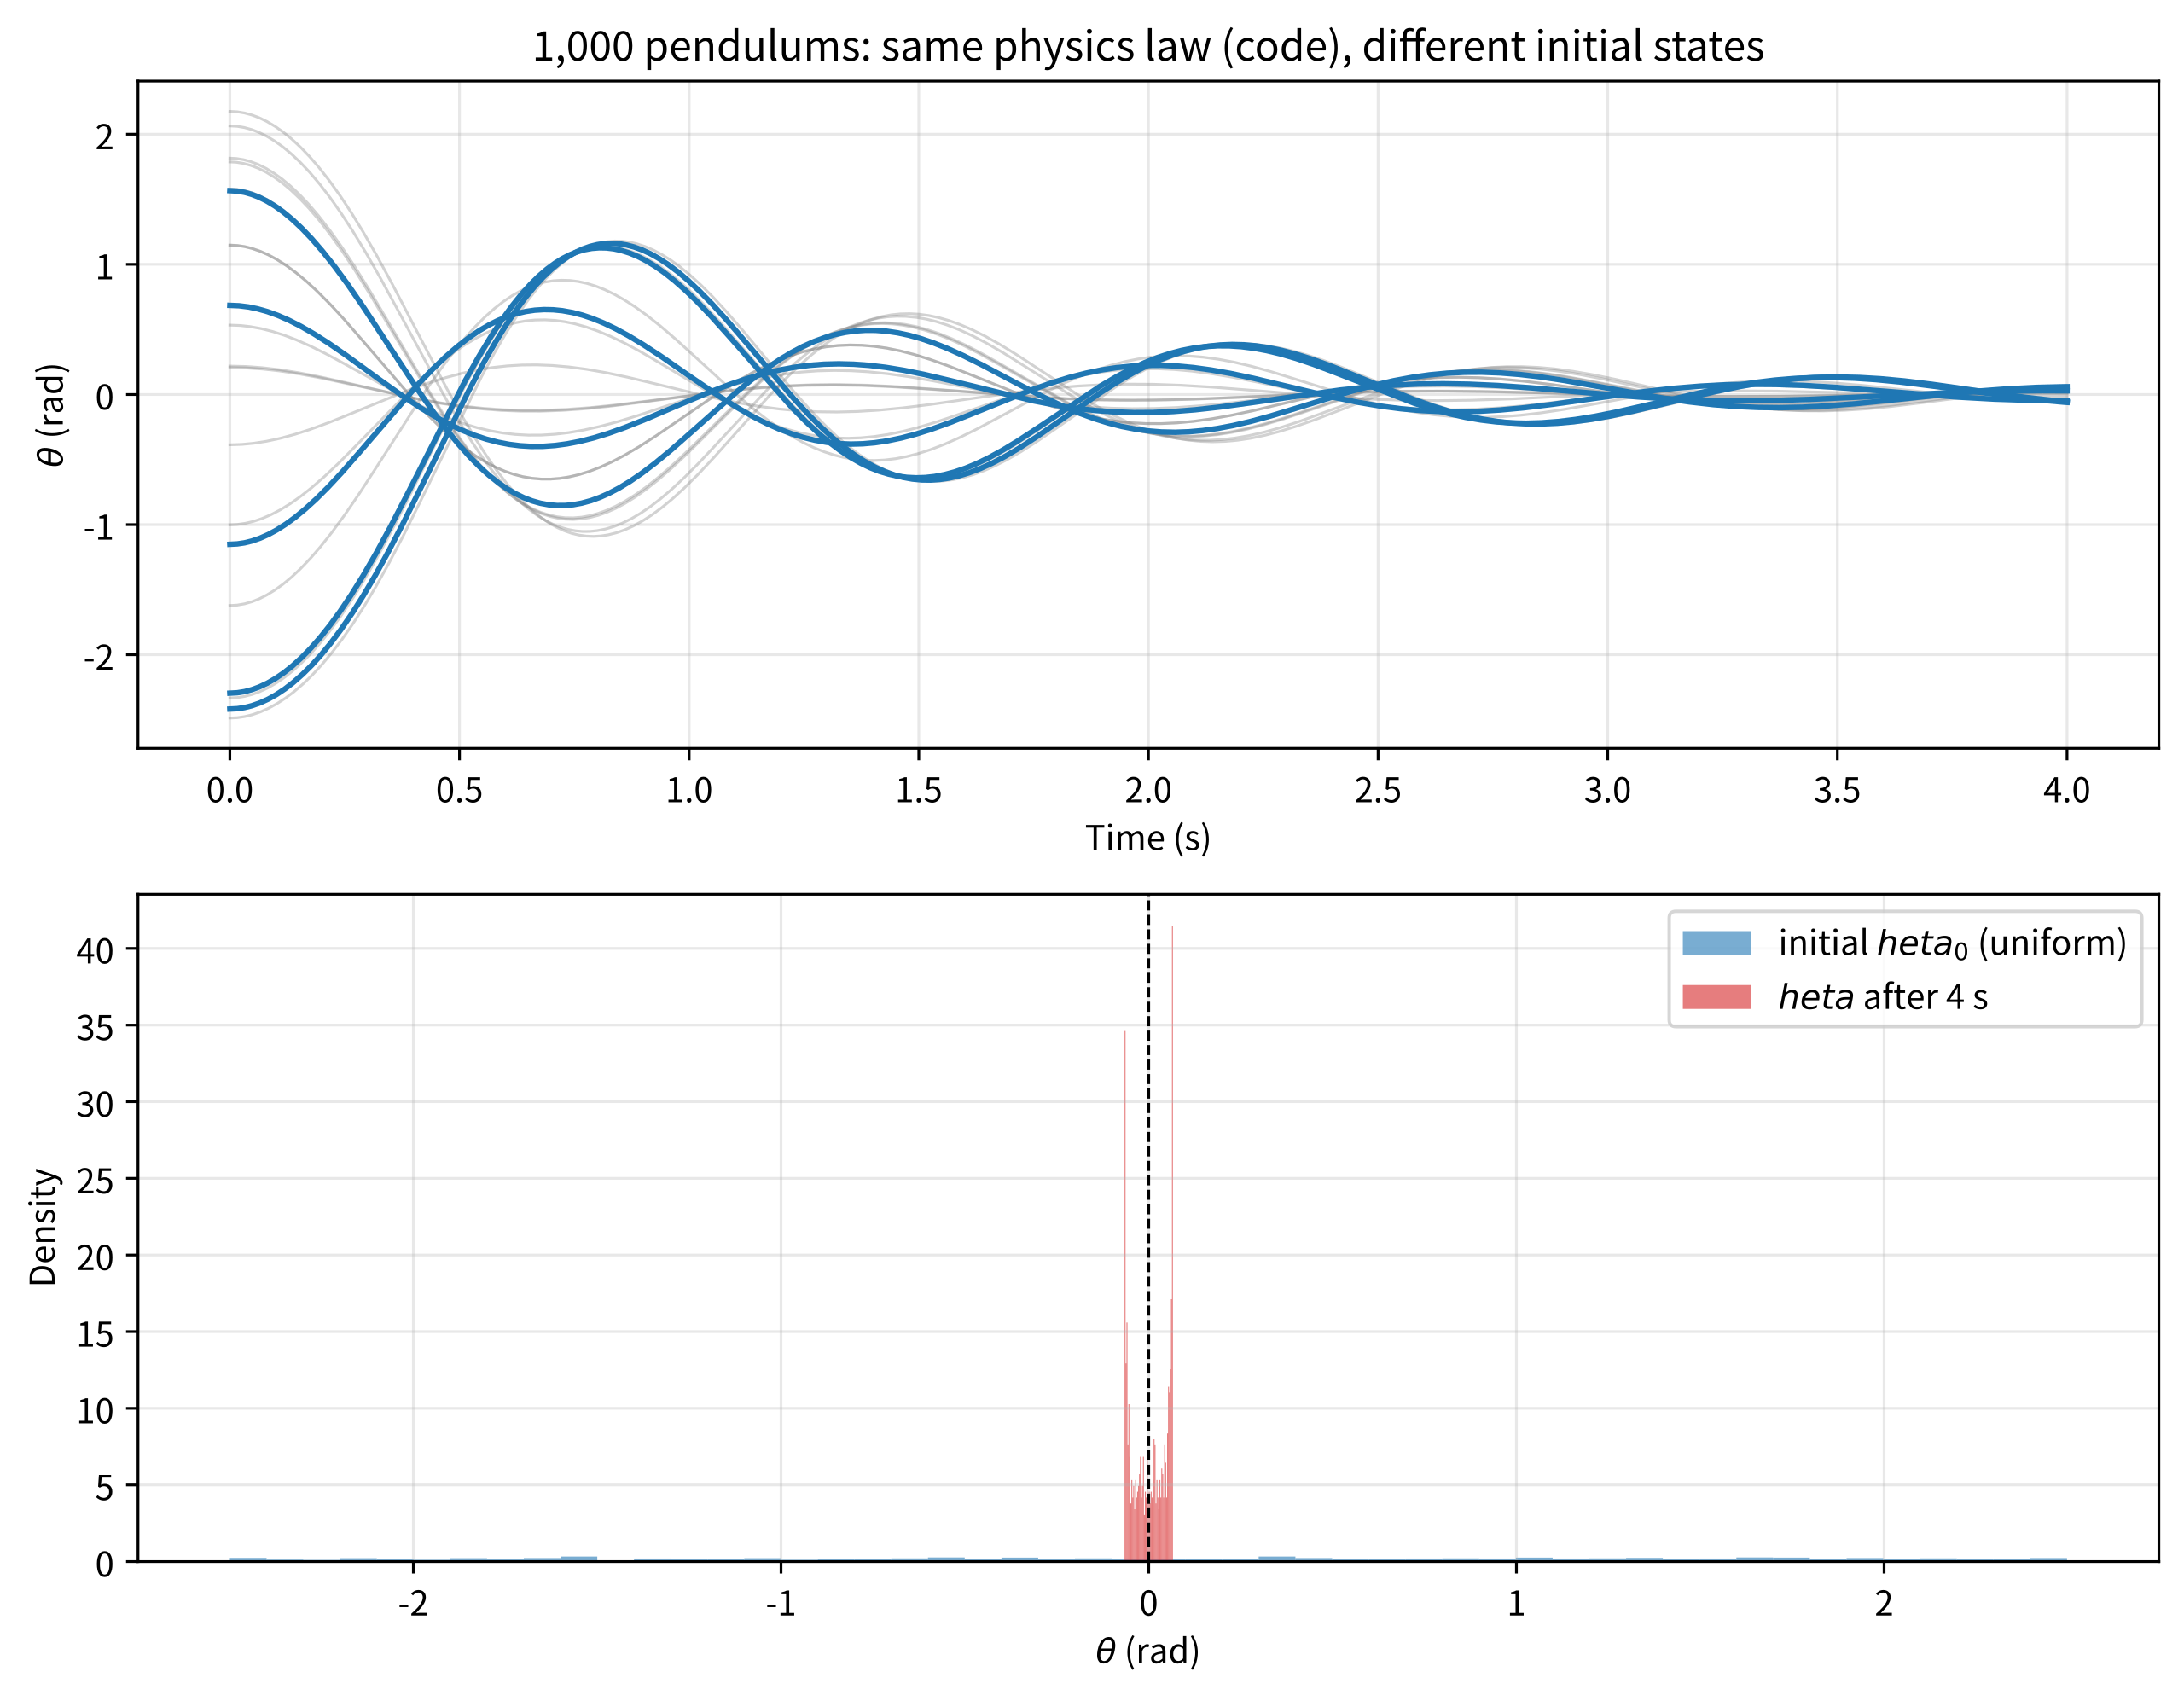
\includegraphics[width=\linewidth]{ch14_2_batch_fan.png}
    \end{column}
    \begin{column}{0.38\textwidth}
      {\footnotesize 1,000개 진자를 $\theta_0 \in [-2.5, 2.5]$에서
      무작위 시작, PD 토크로 2,000스텝(=4s). 모든 궤적이
      \textbf{같은 물리 법칙}(같은 코드)을 따르되, \textbf{출발점}이
      궤적의 모양으로 남는다 --- 하단 분포가 $\theta_0$ 균등분포
      $\to$ 4초 뒤 0 중심으로 수렴.}
    \end{column}
  \end{columns}
\end{frame}

\begin{frame}{``경험률이 1,000배가 되는가?''}
  이 절의 \textbf{가장 중요한 개념적 분기점}.
  답: \kb{환경 스텝 기준으로는 예, 정책 업데이트 기준으로는 아니오}.
  \vskip0.6em
  \begin{columns}[T]
    \begin{column}{0.5\textwidth}
      \kb{(1) 환경 스텝}
      \begin{itemize}
        \item 4s 시뮬레이션의 벽 시간: CPU 순차 1개 진자
          약 0.008s $\times$ 1,000 = 8s(순차 1,000개)
          $\to$ 배치 \textbf{약 0.11s}
        \item 경험 \textbf{수집 속도} 약 \textbf{76배}
          (위 실측) $\Rightarrow$ Ch.\,9 경험재현 버퍼가
          ``순식간에 채워지는'' 이유
      \end{itemize}
    \end{column}
    \begin{column}{0.5\textwidth}
      \kb{(2) 정책 업데이트}
      \begin{itemize}
        \item 1,000개 궤적이 동시에 모였다고, 그 1,000개 트랙을
          정책 그래디언트에 \textbf{한 번에 쓸 수는 없다}
        \item Ch.\,11.2 PPO 미니배치는 \textbf{연속된} (상태,
          행동, 리턴) 튜플을 요구 --- 1,000개 독립 트랙을 하나로
          묶으면 각 트랙 리턴이 자기 초깃값 분포에서 와서
          \textbf{분산이 커짐} (GAE가 일부 처리)
      \end{itemize}
    \end{column}
  \end{columns}
  \vskip0.5em
  \begin{block}{결론}
    GPU 병렬은 \textbf{``경험을 모으는 속도''}를 키우고,
    \textbf{``경험을 쓰는 효율''은 별개 축}. 14.3에서 정확히
    이 둘을 독립 축으로 정리한다.
  \end{block}
\end{frame}

\begin{frame}{자주 하는 실수 (1): ``코어가 많으니까 자동으로 빨라진다''}
  \small
  \begin{tabular}{@{}p{4.6cm}p{9.4cm}@{}}
    \toprule
    실수 & 왜 틀린가 \\
    \midrule
    ``GPU 코어가 16,384개니까 16,384배 빠진다'' &
      \kb{Amdahl}: 순차 부분(동기화, VRAM$\leftrightarrow$host
      복사, 정책 업데이트)이 병렬화되면 \textbf{상수로 묶임}.
      환경 스텝만 볼 때 이론적 상한은 코어 수지만, 전체
      파이프라인(경험 수집 $\to$ 미니배치 $\to$ 업데이트)의
      속도는 \textbf{병렬화 불가 부분}이 정한다. 실제 Isaac Sim
      벤치마크도 ``환경 스텝 $\times$수천''이지 ``$\times$16,384''
      가 아니다 \\
    \bottomrule
  \end{tabular}
  \vskip0.5em
  {\footnotesize 실수 2: ``\textbf{배치(텐서)로 모으는 것 = GPU
  병렬}'' --- 배치는 \textbf{필요조건}이지 \textbf{충분 조건}이
  아님. numpy가 CPU에서 벡터화해도 코어는 8$\sim$16개. GPU가 그
  같은 배치를 수천 코어로 동시 실행해야 \textbf{진짜 GPU 병렬}.
  ``배치로 썼으니까 빠르다''는 CPU 76배(numpy 벡터화 + 오버헤드
  제거)와 GPU 수천 배를 \textbf{혼동}.}
\end{frame}

\begin{frame}{자주 하는 실수 (2): 미니배치와 규모}
  \small
  \begin{tabular}{@{}p{4.6cm}p{9.4cm}@{}}
    \toprule
    실수 & 왜 틀린가 \\
    \midrule
    ``1,000개 환경이 동시에 돌면 PPO 미니배치도 1,000개가
      된다'' & 미니배치는 \textbf{연속된 트랙}의 (s,a,G) 튜플을
      묶는 것. 1,000개 독립 트랙을 하나로 묶으면 \textbf{분산이
      커지고} GAE의 편향-분산 tradeoff가 달라짐. 실무에서는
      경험 수집을 1,000배 빨리하고, \textbf{미니배치 크기는
      알고리즘이 요구하는 크기로 유지} (수집을 빨리 $\to$
      같은 미니배치 크기로 \textbf{더 자주} 업데이트) \\
    ``GPU가 빠르니까 CartPole 실습도 GPU로'' & CartPole 24만
      steps/s $\times$ 책의 12만 스텝 = \textbf{0.5초}. GPU로
      옮겨도 최소 오버헤드(데이터 복사, 동기화) 때문에 \textbf{오히려
      느려질} 수 있음. GPU 병렬의 값은 \textbf{총 스텝 수가 CPU에서
      수 시간$\sim$날 단위가 될 때}(1억+, 14.3)만 드러남 ---
      \textbf{규모 미만의 작업에 GPU는 과잉} \\
    \bottomrule
  \end{tabular}
\end{frame}

\begin{frame}{공통 원리}
  \begin{block}{GPU 병렬을 결정하는 것}
    ``코어 수 $\times$ 데이터 길이''가 아니라,
    \textbf{``병렬화 가능한 부분 $\times$ 코어 수''}로 결정된다.
  \end{block}
  \vskip0.5em
  \begin{itemize}
    \item ``순차 부분''이 \textbf{작을수록}(환경 스텝이 대부분이고,
      동기화가 스텝 경계마다 한 번이면) $\to$ 이 곱에 \textbf{가깝}
    \item ``순차 부분''이 \textbf{크면}(정책 업데이트가 환경 스텝과
      1:1이면) $\to$ Amdahl 상한이 \textbf{훨씬 낮}아진다
  \end{itemize}
  \vskip0.6em
  {\footnotesize 확인 문제 예시: 환경 스텝 99\%($p=0.99$) + 정책
  업데이트 1\%인 시뮬레이터에서 1,000코어 병렬화 후 전체 가속
  $= 1/((1-p)+p/N) \approx 990$배, $N\to\infty$ 상한 = 100배.
  (힌트: $1/((1-p)+p/N)$, $p=0.99, N=1000$)
  }
\end{frame}

\begin{frame}{역사: CUDA에서 Isaac Sim까지}
  Isaac Sim의 ``GPU로 수천 개를 동시에''는 새것이 아니다:
  \small
  \begin{tabular}{@{}p{3.0cm}p{4.6cm}p{6.4cm}@{}}
    \toprule
    단계 & 시점 & 내용 \\
    \midrule
    \kb{CUDA} & 2007 & ``GPU 코어에 데이터를 나란히 놓고,
      커널을 \textbf{한 번} 호출하면 수천 개 코어가 동시에
      수행''하는 프로그래밍 모델 공개 --- 그전 GPU는 렌더링
      전용 \\
    \kb{MuJoCo-XLA} & 2021 (Todorov 등) & 14.1의 MuJoCo를
      TPU/GPU로 \textbf{자동 병렬화} --- 정밀 물리(LCP 접촉)를
      그 구조에 자동 이동 \\
    \kb{Isaac Sim} & 2023 (NVIDIA) & 로봇 시뮬레이터 \textbf{전체}
      (물리 + 렌더링 + 센서)를 그 모델 위로 상품화 \\
    \bottomrule
  \end{tabular}
  \vskip0.6em
  \begin{block}{한 줄 요약}
    세 단계 모두 ``\textbf{공유하는 것은 코드, 달라지는 것은
    상태}''라는 같은 뼈대 위에, \textbf{순차 부분을 줄이고 배치
    크기를 크게} 하는 엔지니어링의 진화.
  \end{block}
\end{frame}

\begin{frame}{``RT 코어가 필요하다''는 제약의 정확한 이유}
  \begin{itemize}
    \item Isaac Sim은 물리만 GPU로 돌리는 게 아니라,
      \textbf{렌더링(카메라 센서 시뮬레이션)까지} GPU에서
    \item 실시간 렌더링을 위해 광선 추적(ray tracing)을 쓰면
      GPU의 \textbf{RT 코어} 필요 --- A100\,·\,H100류 데이터센터
      GPU는 학습용이라 RT 코어가 \textbf{없음}
  \end{itemize}
  \vskip0.6em
  \begin{block}{정확한 이유}
    ``학교 GPU(H100)로 Isaac Sim을 못 돌린다''는 제약은
    \textbf{렌더링 축(시각적 리얼리즘)}에서 온다.
    \textbf{물리만이라면 MuJoCo-XLA로 H100에서도 돌릴 수 있다}
    --- ``GPU가 없어서 못 한다''가 아니라,
    \textbf{``렌더링을 하려면 이 GPU가 아니다''}라는 정확한
    이유 (14.3의 Q3가 이 지점을 다룬다).
  \end{block}
\end{frame}

\begin{frame}{자주 묻는 질문 (14.2)}
  \small
  \begin{itemize}
    \item \textbf{Q. GPU 가속에서도 DQN/PPO를 그대로?}
      \textbf{그렇다} --- 알고리즘은 ``환경이 한 번에 경험을
      몇 개 주는가''와 무관하게 정의. 다만 실전 구현은 수천 개
      복제본 데이터를 \textbf{한꺼번에 배치로} 처리하도록 최적화
      (Ch.\,9.3 미니배치 개념의 자연스러운 확장) --- 알고리즘
      수학은 그대로, 구현만 조정.
    \item \textbf{Q. Isaac Sim을 못 써본 건 손해인가?}
      \textbf{개념적으로는 크지 않다} --- 핵심 가치는
      ``같은 알고리즘을 훨씬 빠르게 많이 학습''시키는
      \textbf{계산 효율성}이지, 새 알고리즘을 배우게 하는 게
      아님. MuJoCo로 배운 워크플로가 나중에 적합한 GPU가
      생기면 \textbf{그대로 Isaac Sim으로, 규모만 키워} 이식.
  \end{itemize}
\end{frame}

\begin{frame}{자주 묻는 질문 (14.2): ``한 번''이 진짜 한 번인가}
  \begin{itemize}
    \item \textbf{Q. 4,096개 환경이 \textbf{진짜} 동시에인가?}
      구조적으로는 \textbf{``한 번''} --- 호출은 한 번, 그 안에서
      수천 개 코어가 \textbf{동시에} 수행.
    \item 물리적으로: GPU의 SM(Streaming Multiprocessor)이
      \kb{워프}(32개 스레드) 단위로 스케줄링 $\Rightarrow$
      4,096개 환경이 \textbf{완벽히} 동시에 끝나는 건 아님 ---
      대부분이 동시에, 일부는 \textbf{다음 워프 스케줄링}에서
    \item 하지만 호출 오버헤드가 \textbf{일단}만 치러지므로,
      순차 4,096회 호출에 비해 총 시간은 \textbf{수천 분의 1}
  \end{itemize}
  \vskip0.5em
  \begin{block}{핵심}
    ``\textbf{완벽한 동시성}''이 아니라,
    \textbf{``호출 오버헤드를 상수로 묶는다''}는 것이 핵심.
  \end{block}
  \vskip0.4em
  {\footnotesize Q. MuJoCo-XLA vs Isaac Sim? 둘 다 ``정밀 물리를
  GPU/TPU로 병렬화''하지만 \textbf{범위}가 다름: MuJoCo-XLA =
  물리만(LCP 포함, 렌더링 없음, CPU MuJoCo와 \textbf{완전히 같은
  물리}). Isaac Sim = 물리+렌더링+센서(RT 코어 필요, 물리 엔진도
  NVIDIA Warp 기반). ``정밀 물리만 GPU로''면 MuJoCo-XLA,
  ``물리+카메라로 판단하는 정책''이면 Isaac Sim.
  }
\end{frame}

\section{14.3 어떤 도구를 언제 쓰는가}

\begin{frame}{원리가 아니라 숫자로}
  \begin{itemize}
    \item 14.1: MuJoCo 직접 다룸 / 14.2: Isaac Sim GPU 병렬 원리
    \item 이번 절: ``어떤 작업을 어떤 도구로 풀어야 하는가''를
      \textbf{원리가 아니라 숫자}로 정리
  \end{itemize}
  \vskip0.6em
  \textbf{이 절을 마치면}:
  \begin{enumerate}
    \item \textbf{정밀도 $\cdot$ 속도}라는 \textbf{두 개의 축}으로
      도구를 비교하는 눈
    \item 내 작업이 그 두 축에서 \textbf{어디에 찍히는지} 재는
      방법
    \item 30초 안에 도구를 고르는 \kb{결정 절차}
  \end{enumerate}
\end{frame}

\begin{frame}{네 도구를 한 표로}
  \small
  \begin{tabular}{@{}p{3.4cm}p{1.8cm}p{2.2cm}p{3.4cm}p{3.4cm}@{}}
    \toprule
    도구 & 실행 위치 & 정밀도 & 속도(대량 병렬) & 이번 학기 사용 \\
    \midrule
    Gymnasium 기본 & CPU & 낮음$\sim$중간 & 느림 & 기본 실습 \\
    PyBullet & CPU & 중간 & 느림 & 로봇팔/사족보행 실습 \\
    MuJoCo & CPU & 높음 & 느림 & 정밀 제어 실습 \\
    NVIDIA Isaac Sim & GPU & 높음 & 매우 빠름(수천 배
      병렬) & 시연만(하드웨어 제약) \\
    \bottomrule
  \end{tabular}
  \vskip0.7em
  \begin{itemize}
    \item 개인 노트북에서 직접 돌려보고 싶다면 $\to$
      \textbf{Gymnasium/PyBullet}
    \item 접촉·마찰까지 \textbf{정밀하게} 맞춰야 하는 연구라면
      $\to$ \textbf{MuJoCo}
    \item \textbf{대량의 경험}을 매우 빠르게 모아야 하는 대규모
      학습이라면 (그리고 적합한 GPU가 있다면) $\to$
      \textbf{Isaac Sim}
  \end{itemize}
\end{frame}

\begin{frame}{이 절의 뼈대 (두 질문)}
  \begin{block}{핵심 선언}
    시뮬레이션 도구가 달라져도 \textbf{강화학습 알고리즘 자체는
    바뀌지 않는다} --- 바뀌는 건 \textbf{물리적 정확도와 계산
    속도의 트레이드오프}뿐. 어떤 도구를 쓸지는
    \textbf{``얼마나 정밀해야 하는가''}와 \textbf{``얼마나 많은
    경험이 필요한가''}라는 두 질문에 대한 \textbf{답}으로
    결정된다.
  \end{block}
  \vskip0.5em
  \begin{itemize}
    \item 셋 다 Ch.\,9--13 알고리즘을 그대로 얹을 수 있는,
      \textbf{``환경을 바꿔 끼우는''} 문제라는 점은 동일
  \end{itemize}
  \vskip0.4em
  {\footnotesize 아래에서 각 ``질문''이 \textbf{실제로 무엇을
  재는지}를 하나씩 풀고, 둘이 만나는 지점에서 도구를 고르는
  절차를 숫자까지 붙여 다룬다.}
\end{frame}

\begin{frame}{첫 번째 질문: ``얼마나 정밀해야 하는가?''}
  \begin{itemize}
    \item ``정밀도''를 모호한 말이 되지 않게 14.1의
      \kb{접촉(contact)}에서 시작
    \item 공이 바닥에 \textbf{닿는 순간}은 단순 미분방정식이
      아니라 \kb{LCP}라는 특별한 최적화
      (비침투 + 비음이 \textbf{동시에})
  \end{itemize}
  \vskip0.5em
  \begin{itemize}
    \item MuJoCo가 LCP를 매 스텝 안정적으로 풀어:
      (1) 공이 부딪혀 튀다 멈추는 행위가 \textbf{NaN·폭주 없이}
      자연스럽고, (2) 다리 로봇의 발이 바닥에 붙었다 떨어지는
      \textbf{걸음} 같은 복잡한 접촉도 같은 식으로
  \end{itemize}
  \vskip0.5em
  \begin{block}{핵심 정지점}
    \kb{정밀도는 ``화면이 사실적인가''가 아니라, ``정책이 배우는
    물리가 \textbf{진짜와 얼마나 같은가}''}를 말한다.
    두 가지가 \textbf{서로 다른 축}이다.
  \end{block}
\end{frame}

\begin{frame}{두 축: 물리 정밀도 vs 시각적/센서 리얼리즘}
  \begin{columns}[T]
    \begin{column}{0.48\textwidth}
      \kb{물리 정밀도}
      \begin{itemize}
        \item 접촉, 마찰, 관성, \textbf{접촉력(contact force)}이
          물리 법칙에 얼마나 충실한가
        \item \textbf{로봇 제어}에서 이 축이 \textbf{가장 중요}
        \item 다리로 서 있는 로봇의 발이 미끄러지지 않도록 하는
          제어는, \textbf{접촉력이 정확}하게 계산되는 엔진 위에서
          배워야 실제로 \textbf{이식}
        \item 14.1의 ``부딪혀 안착''이라는 \textbf{동역학} 자체가
          이 축의 문제
      \end{itemize}
    \end{column}
    \begin{column}{0.48\textwidth}
      \kb{시각적/센서 리얼리즘}
      \begin{itemize}
        \item 카메라로 본 \textbf{픽셀}이 얼마나 사실적인가
        \item \textbf{시각적으로 판단하는} 정책(픽셀 입력)을 만들
          때 중요
        \item Isaac Sim이 사실적 렌더링을 지원하는 이유가 바로
          이것 --- 14.2의 ``픽셀을 보고 판단하는 로봇 정책''
          대목이 이 축
      \end{itemize}
    \end{column}
  \end{columns}
\end{frame}

\begin{frame}{왜 이 구분이 중요한가}
  \begin{itemize}
    \item ``화면이 예쁘니까'' Isaac Sim을 고르면: 실제로는
      \textbf{물리 정밀도}가 필요한 작업을 \textbf{비싼 GPU}
      위에서 돌리는 셈이 되기 쉬움
    \item 반대로, 접촉력이 정확해야 하는 다리 로보를
      ``CartPole도 되는데''라며 \textbf{가장 단순한 환경}에서
      배우면: 13.1의 \kb{현실 격차(reality gap)}가 그 단순함에서
      \textbf{이미 박혀} 있다 --- 시뮬레이터 자체가 물리를 너무
      약하게 근사하고 있기 때문
  \end{itemize}
  \vskip0.6em
  \begin{columns}[T]
    \begin{column}{0.48\textwidth}
      \kb{축 A: 물리}
      \begin{itemize}
        \item 접촉력 정확도
        \item \textbf{로봇 제어}의 핵심
      \end{itemize}
    \end{column}
    \begin{column}{0.48\textwidth}
      \kb{축 B: 센서}
      \begin{itemize}
        \item 렌더링 리얼리즘
        \item \textbf{픽셀 입력 정책}의 핵심
      \end{itemize}
    \end{column}
  \end{columns}
\end{frame}

\begin{frame}{정밀도 축을 작업별로 대입하면}
  \small
  \begin{tabular}{@{}p{4.6cm}p{2.8cm}p{6.6cm}@{}}
    \toprule
    작업 (Chapter) & 필요한 정밀도 & 이유 \\
    \midrule
    CartPole, Pendulum (9$\sim$11) & 낮음$\sim$중간 &
      단일 막대/진자. 접촉 없음, 물리 근사만으로도 충분 \\
    Reacher, 2관절 로봇팔 (13) & 중간 & 관절 운동은 있지만
      \textbf{자발적인 강한 접촉} 없음 \\
    사족보행/인간형 보행 (13.2) & \textbf{높음} & 발이 바닥에
      \textbf{붙었다 떨어지는} 반복 접촉. 접촉력 정확도가 핵심 \\
    카메라로 판단하는 정책 & 높음(센서) + 물리 & 렌더링
      리얼리즘과 물리 정밀도 \textbf{둘 다} 필요 \\
    \bottomrule
  \end{tabular}
  \vskip0.7em
  \begin{block}{정밀도 축의 결론}
    ``\textbf{접촉이 얼마나 중요한가}''로 결정된다. 접촉이 거의
    없으면(Pendulum) Gymnasium 기본 환경, 관절이 있지만 강한
    접촉이 없으면(Reacher) PyBullet/MuJoCo 어느 쪽이든 충분,
    \textbf{발이 바닥을 차는 보행}이라면 MuJoCo급 정밀 LCP
    접촉이 \textbf{필수}.
  \end{block}
\end{frame}

\begin{frame}{두 번째 질문: ``얼마나 많은 경험이 필요한가?''}
  \begin{itemize}
    \item ``속도''는 모호한 ``빠르다''가 아니라,
      \textbf{초당 몇 번의 (상태, 행동, 보상) 경험을 모을 수 있는가}
    \item 이 정의가 중요한 이유: Ch.\,9--13의 \textbf{모든}
      알고리즘이 결국 이 경험 데이터를 \textbf{먹고} 작동
  \end{itemize}
  \vskip0.5em
  \begin{enumerate}
    \item \kb{경험재현 버퍼}(Ch.\,9.3): 버퍼가 차야 미니배치
      샘플링 시작
    \item \kb{GAE}(Ch.\,11.2): 에피소드 \textbf{분할}을 모아야
      보너(bootstrapping) 값을 추정
    \item \kb{PPO} 정책 그래디언트: 충분한 수의 (상태, 행동,
      리턴) 트플 위에서 그래디언트 하강
  \end{enumerate}
  \vskip0.5em
  \begin{block}{결론}
    알고리즘이 필요로 하는 \textbf{총 경험 수}가 정해지면,
    \textbf{초당 스텝 수가 그 학습의 실시간 길이를 결정}.
  \end{block}
\end{frame}

\begin{frame}{실측(학교 서버 CPU, 2026-08)}
  먼저 \textbf{책에서 실제로 돌린} 실행의 총 스텝 수:
  \small
  \begin{tabular}{@{}p{4.4cm}p{3.0cm}p{6.0cm}@{}}
    \toprule
    실행 & 총 스텝 수 & 계산 \\
    \midrule
    11.2 Pendulum PPO & 120,000 & 300 iter $\times$ 400 스텝 \\
    13.3 Reacher PPO & 76,800 & 150 iter $\times$ 512 스텝 \\
    \bottomrule
  \end{tabular}
  $\Rightarrow$ 이 책의 PPO 실습들은 \textbf{약 8만$\sim$12만 스텝}이면
  ``배우는 것''이 끝남. 이제 각 엔진의 초당 스텝 수로 나누면:
  \small
  \begin{tabular}{@{}p{5.6cm}p{3.6cm}p{4.8cm}@{}}
    \toprule
    엔진 (환경) & 초당 스텝 수 & 120,000 스텝에 걸리는 시간 \\
    \midrule
    Gymnasium 기본 (CartPole-v1) & 약 247,000 & 약 \textbf{0.5 초} \\
    MuJoCo (Ant-v5) & 약 6,200 & 약 \textbf{20 초} \\
    \bottomrule
  \end{tabular}
  {\footnotesize 노트북 재현: \texttt{gym.make(...)} 후
  \texttt{step()} 반복 + \texttt{time.perf\_counter()}, 워밍업
  200스텝 제외. 이 숫자는 \textit{이 책의 실습 수준}에서 CPU의
  절대 상한선을 재는 것.}
\end{frame}

\begin{frame}{표 읽는 법: ``CPU니까 느리다''가 아니다}
  \begin{block}{같은 CPU에서 40배}
    가장 단순한 환경(CartPole, 물리 근사)이 가장 정밀한 로봇
    시뮬레이션(Ant, MuJoCo)보다 \textbf{약 40배 빠름}.
    ``CPU니까 느리다''가 아니라, \textbf{정밀한 물리를 계산하는
    \textit{비용}이 CPU를 40배 느리게 만든다} --- 14.1에서 LCP
    접촉을 매 스텝 푸는 데 드는 계산이 이 차이의 정체.
  \end{block}
  \vskip0.6em
  \begin{columns}[T]
    \begin{column}{0.56\textwidth}
      \centering
      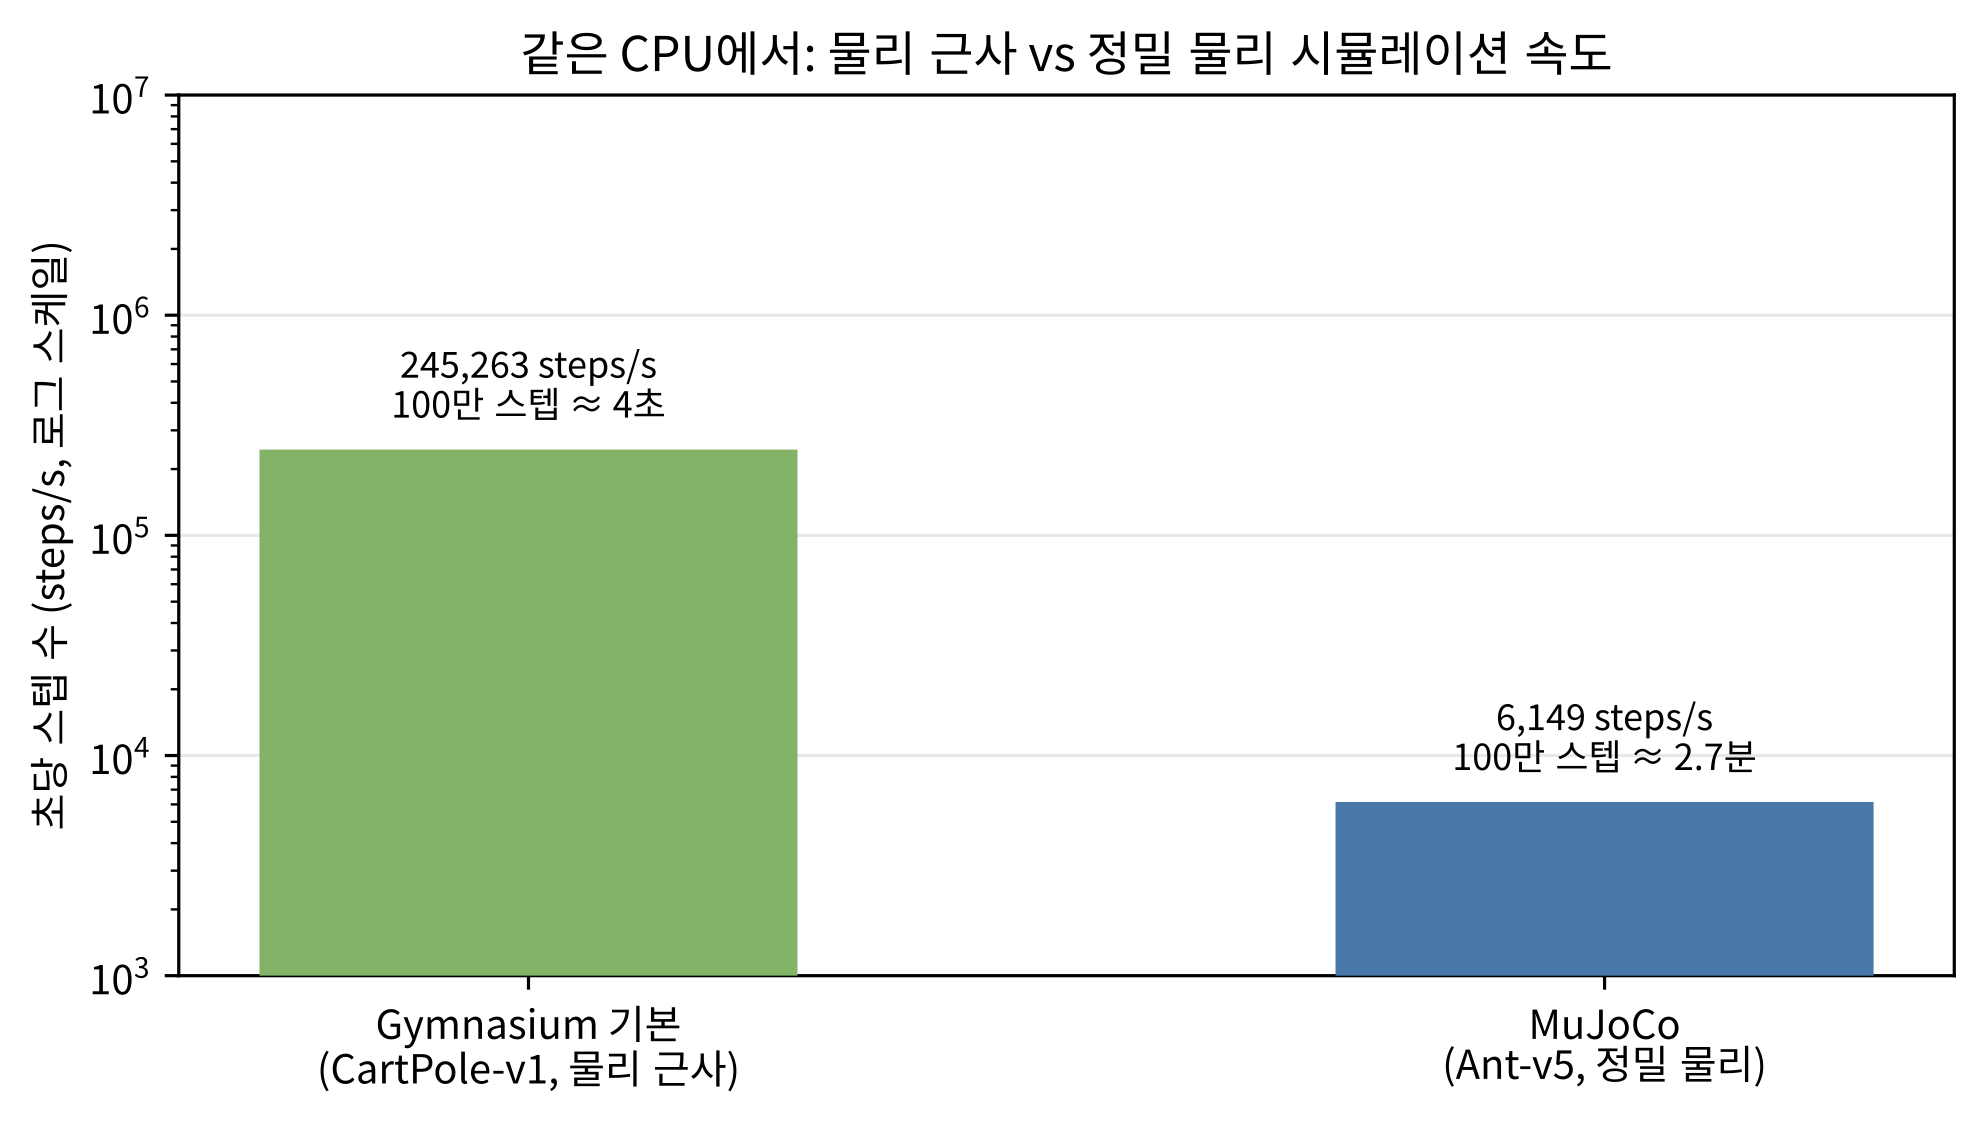
\includegraphics[width=\linewidth]{ch14_3_engine_speed.png}
    \end{column}
    \begin{column}{0.40\textwidth}
      {\footnotesize 초당 스텝 수 비교(로그 스케일). CartPole
      $\approx$247,000 steps/s, Ant $\approx$6,200 steps/s.
      100만 스텝에 걸리는 시간: CartPole $\approx$ \textbf{4초},
      Ant $\approx$ \textbf{2.7분} --- 둘 다 ``CPU''인데
      \textbf{어떤 물리를 계산하느냐}에 따라 40배로 갈린다.
      ``느림''의 크기를 실감하라.}
    \end{column}
  \end{columns}
\end{frame}

\begin{frame}{규모를 단계별로: 총 스텝 수 $\div$ 초당 스텝 수}
  \kb{환경 스텝만}의 실 시간(오른쪽은 14.2의 ``수천 개 복제본
  동시 스텝''을 \textbf{경험률 2,000배}로 단순화한 GPU 병렬):
  \small
  \begin{tabular}{@{}p{3.8cm}p{4.2cm}p{4.6cm}@{}}
    \toprule
    총 스텝 수 & 단일 CPU (Ant) & GPU 병렬 $\times$2,000 \\
    \midrule
    책의 PPO (약 12만) & 약 \textbf{20 초} & (CPU면 충분) \\
    사족보행 (1,000만) & 약 \textbf{27 분} & 약 0.8 초 \\
    대규모 보행 (1억) & 약 \textbf{4.5 시간} & 약 8 초 \\
    초대규모 (10억) & 약 \textbf{2 일} & 약 1.3 분 \\
    \bottomrule
  \end{tabular}
  \vskip0.5em
  {\footnotesize ``GPU $\times$2,000''는 \textbf{환경 스텝}의
  병렬화일 뿐 --- 정책 네트워크의 순전파·그래디언트 계산은
  \textbf{별도} (바로 아래 ``확인'').
  }
\end{frame}

\begin{frame}{이 표가 이 절의 핵심}
  \begin{itemize}
    \item 책의 12만 스텝은 CPU 한 대면 \textbf{20초} ---
      \textbf{개인 노트북 + CPU로 이번 학기 실습을 \textit{전부}
      할 수 있다}. 이것이 ``이번 학기 실습은 MuJoCo를 기본으로
      골랐다''는 FAQ의 \textbf{계산적 근거}
  \end{itemize}
  \vskip0.6em
  \begin{block}{반전}
    같은 Ant가 \textbf{10억 스텝}이면: 단일 CPU \textbf{약 2일},
    GPU 병렬은 \textbf{약 1.3분}. GPU 병렬의 ``수천 배''라는 값은
    \textbf{10만 스텝이 아니라 1억$\sim$10억 스텝}에서야 비로소
    ``2일짜리 작업''과 ``몇 분짜리 작업''의 차이가 된다.
  \end{block}
  \vskip0.6em
  \begin{block}{속도 축의 결론}
    ``\textbf{총 스텝 수 $\div$ 초당 스텝 수 = 실 시간}''이고,
    이 실 시간이 \textbf{내가 기다릴 수 있는 범위}(분$\sim$수
    시간)를 넘는 규모(여기선 \textbf{1억 스텝 이상}, 환경 스텝만
    수 시간)에서만 \textbf{GPU 병렬이 필수}. 그 이하 규모에서는
    CPU 정밀(MuJoCo)이 더 느리지만 \textbf{기다릴 만한} 시간이니,
    ``\textbf{정밀도 우선}''이 그대로 합리적 선택.
  \end{block}
\end{frame}

\begin{frame}{확인: ``초당 스텝 수''와 ``학습 효율''은 같은가}
  \begin{block}{아니다}
    초당 스텝 수는 \textbf{경험을 모으는 속도}일 뿐, 그 경험이
    \textbf{얼마나 잘 쓰이는가}(정책 그래디언트의 품질, 버퍼
    재사용률 등)는 \textbf{별개의 문제}.
    GPU가 경험을 1,000배 빨리 모아도, 알고리즘이 그 경험을
    0.1배의 효율로만 쓴다면 \textbf{순} 학습 시간은 \textbf{100배}
    가 된다.
  \end{block}
  \vskip0.6em
  \begin{itemize}
    \item Ch.\,9의 ``경험재현''이 경험을 \textbf{재사용}해 효율을
      높이는 기법인 이유가 바로 이것
    \item \kb{GPU}가 ``\textbf{빠르게 모으는}'' 축,
      \kb{경험재현}이 ``\textbf{효과적으로 쓰는}'' 축을 담당
  \end{itemize}
  \vskip0.5em
  \begin{block}{독립 축}
    이 두 축이 \textbf{독립}해서 \textbf{곱해져} 총 학습 시간을
    만든다.
  \end{block}
\end{frame}

\begin{frame}{30초 결정 절차: 두 축이 만나는 지점}
  \begin{columns}[T]
    \begin{column}{0.52\textwidth}
      \centering
      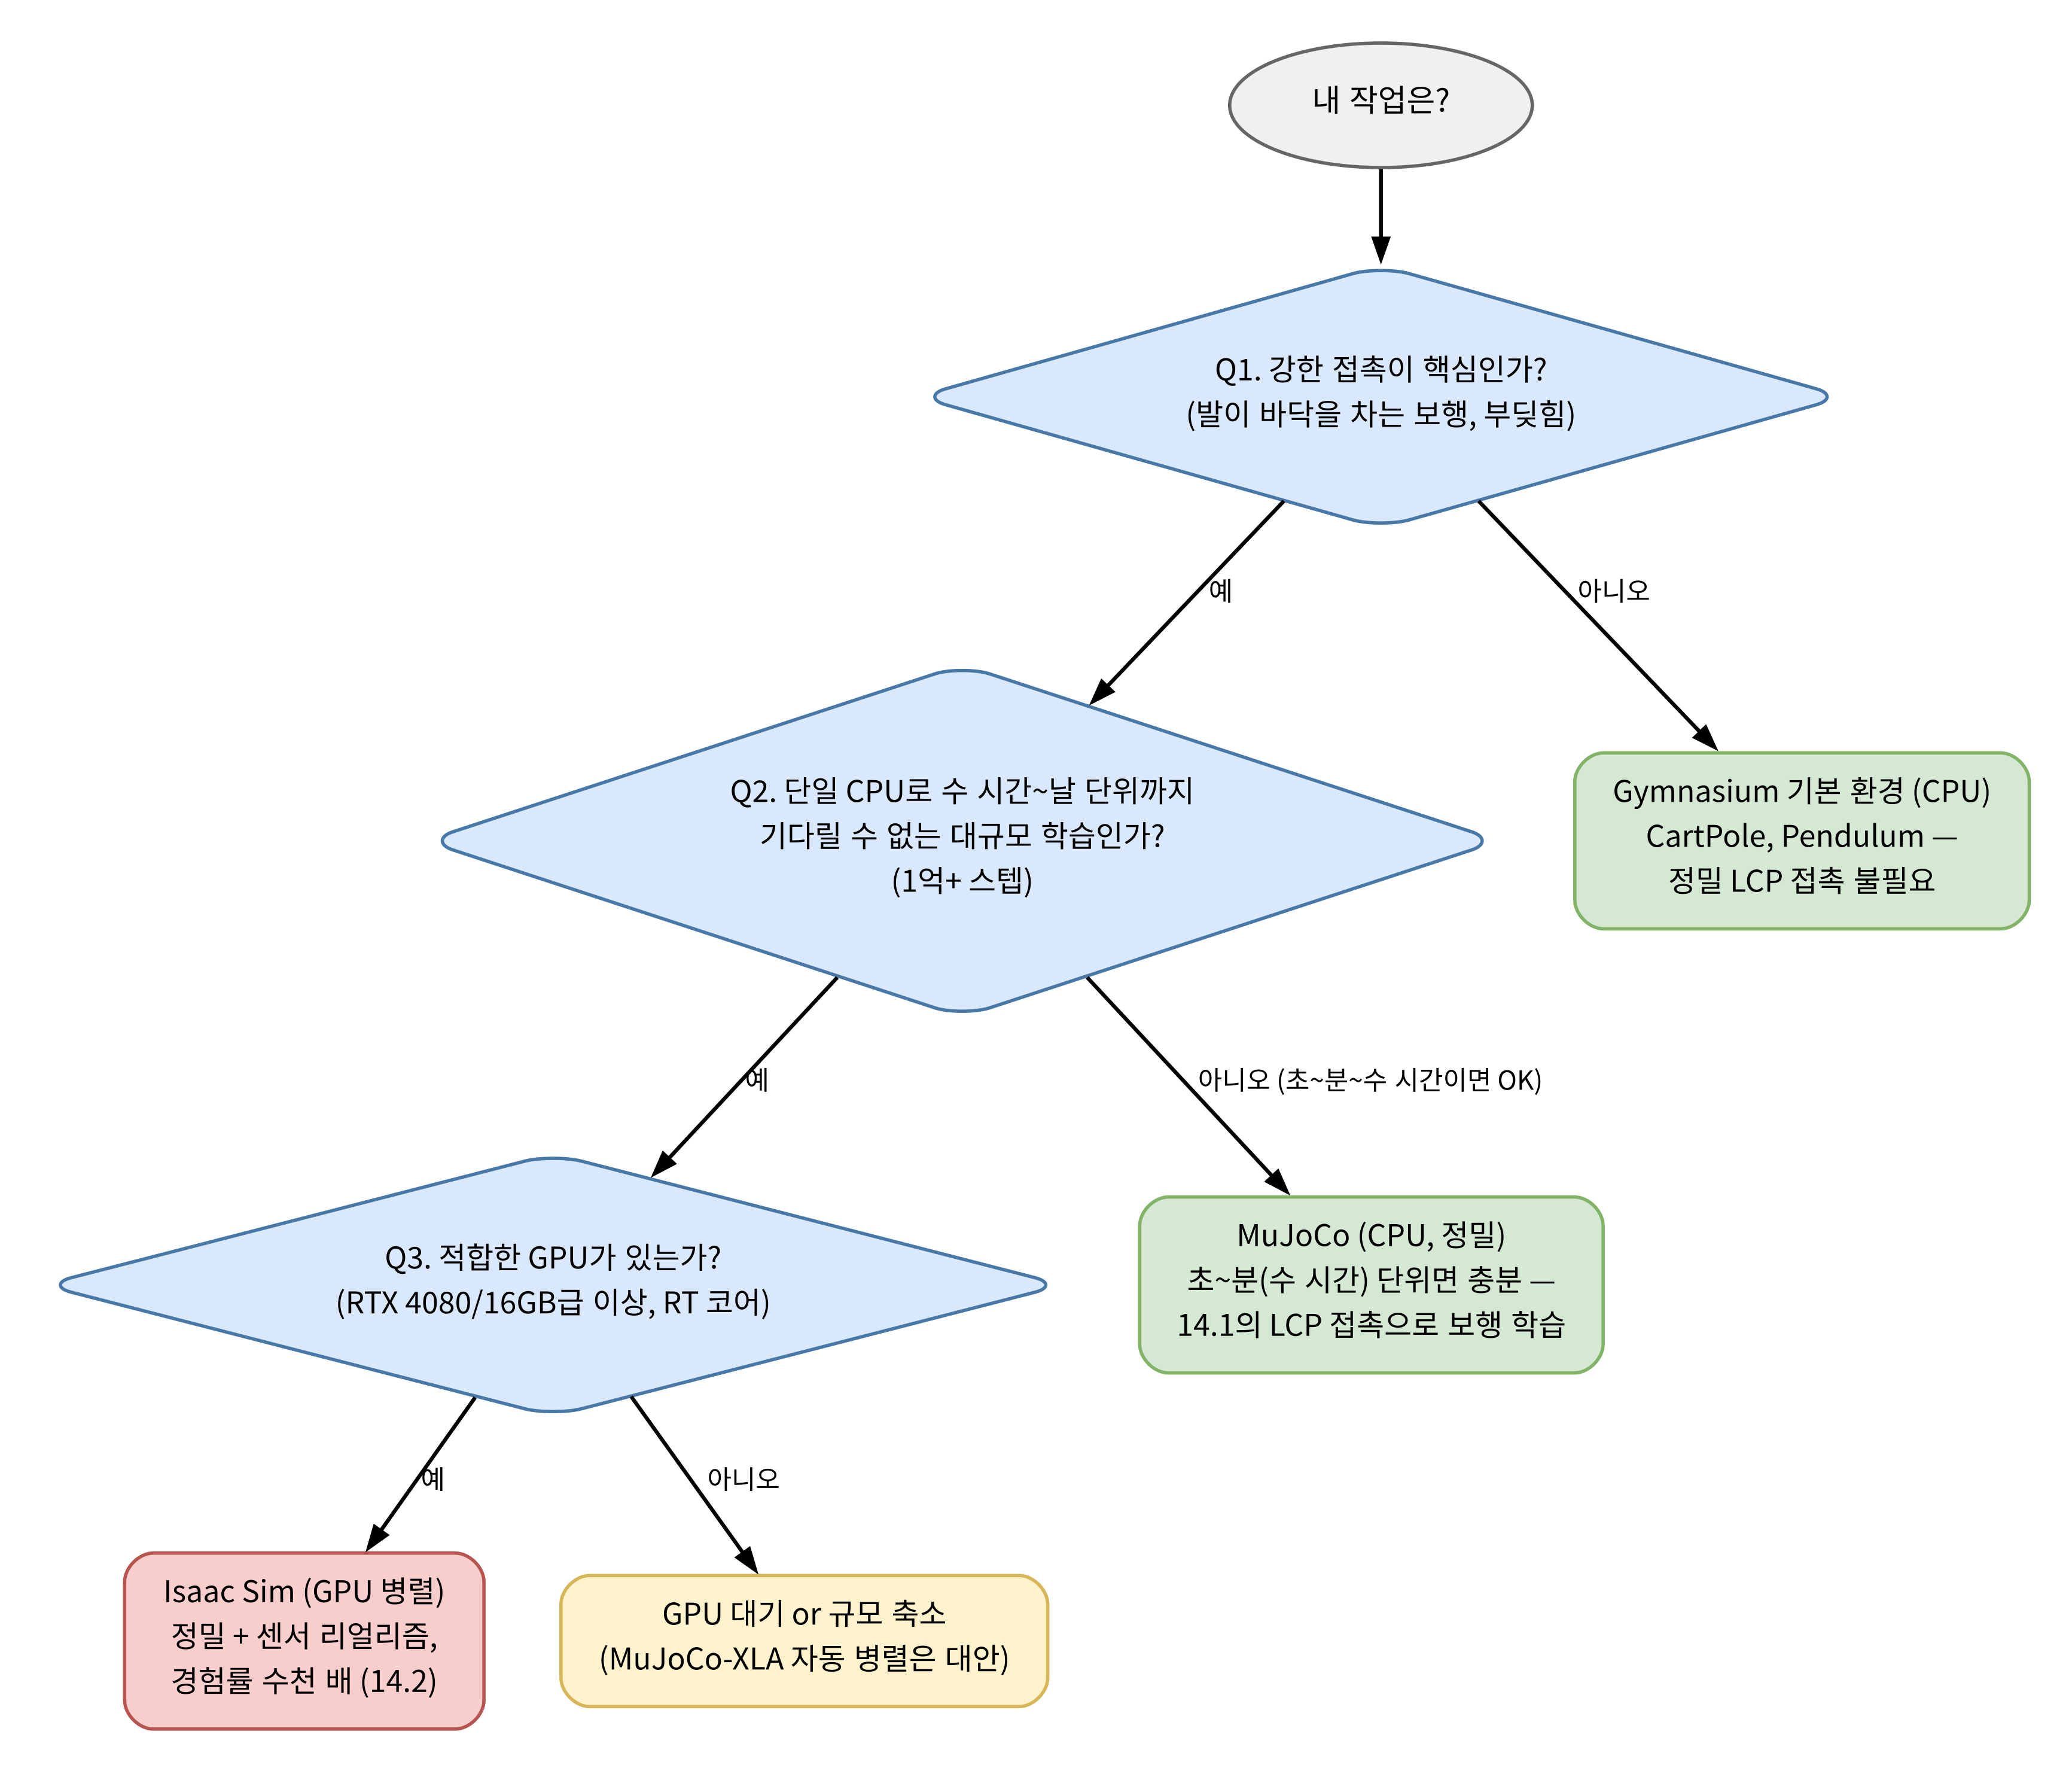
\includegraphics[width=\linewidth]{ch14_3_tool_decision.png}
    \end{column}
    \begin{column}{0.44\textwidth}
      \kb{Q1. 강한 접촉이 핵심인가?}
      발이 바닥을 차는 보행, 물체가 부딪혀 튕기는 조작이
      \textbf{핵심}인가?
      \begin{itemize}
        \item \textbf{아니오} $\to$ 정밀 LCP 접촉 불필요 $\to$
          \textbf{Gymnasium 기본 환경} (CartPole, Pendulum)
        \item \textbf{예} $\to$ 다음
      \end{itemize}
      \kb{Q2. 단일 CPU로 수 시간$\sim$날 단위까지 기다릴 수 없는
      대규모(1억+ 스텝)인가?}
      \begin{itemize}
        \item \textbf{아니오} (초$\sim$분$\sim$수 시간이면 OK ---
          책의 12만 스텝, 1,000만도 CPU 27분(환경 스텝만))
          $\to$ \textbf{MuJoCo (CPU, 정밀)}
        \item \textbf{예} $\to$ 다음
      \end{itemize}
      \kb{Q3. 적합한 GPU가 있는가?} (Isaac Sim: RTX 4080/16GB급
      이상, RT 코어 필요 --- 14.2)
      \begin{itemize}
        \item \textbf{예} $\to$ \textbf{Isaac Sim (GPU 병렬)}
        \item \textbf{아니오} $\to$ GPU 대기, or
          \textbf{MuJoCo-XLA} 자동 병렬, or MuJoCo(CPU)로
          \textbf{규모 축소}
      \end{itemize}
    \end{column}
  \end{columns}
\end{frame}

\begin{frame}{왜 정밀도(Q1)가 첫 질문인가}
  \begin{block}{정밀도 = 필요충분 조건, 속도 = 비용 절감}
    정밀도(Q1)가 \textbf{필수 조건}이기 때문 --- 정밀도가 부족하면
    그 이상 속도가 빨라도 \textbf{잘못된 물리를 빠르게} 배우는
    것(13.1의 현실 격차가 그 출발점). 정밀도가 \textbf{충족된
    이후}에야 속도(Q2, Q3)가 ``어느 CPU/GPU''의 선택이 된다.
  \end{block}
  \vskip0.6em
  \begin{columns}[T]
    \begin{column}{0.48\textwidth}
      \kb{정밀도 (Q1)}
      \begin{itemize}
        \item \textbf{필수 조건} --- 부족하면 속도 무의미
        \item ``잘못된 물리를 빠르게 배우는'' 것을 막음
      \end{itemize}
    \end{column}
    \begin{column}{0.48\textwidth}
      \kb{속도 (Q2, Q3)}
      \begin{itemize}
        \item 정밀도 충족 \textbf{이후}의 선택
        \item ``어느 CPU/GPU''를 쓸지의 \textbf{비용 절감} 문제
      \end{itemize}
    \end{column}
  \end{columns}
\end{frame}

\begin{frame}{자주 하는 실수: CartPole 벤치마크로 ``CPU면 충분''}
  \small
  \begin{tabular}{@{}p{4.8cm}p{9.2cm}@{}}
    \toprule
    실수 & 왜 틀린가 \\
    \midrule
    ``CartPole로 247,000 steps/s를 보고 CPU는 25만 스텝/초니까
      빠르다'' & 그 숫자는 \textbf{물리 근사} 환경의 속도. 정밀
      로봇(Ant)은 같은 CPU에서 \textbf{40배 느린} 6,200 steps/s.
      \textbf{어떤 물리를 계산하느냐}가 속도를 정한다 \\
    ``화면이 사실적이니까'' Isaac Sim을 정밀 제어 작업에 &
      \textbf{시각적 리얼리즘(렌더링)} $\neq$ \textbf{물리
      정밀도}. 접촉력이 정확한 작업은 \textbf{물리 정밀도}가
      필요, 렌더링은 \textbf{센서 축} \\
    GPU가 1,000배 빠르다며 책의 8만 스텝 실습도 GPU로 & 8만
      스텝은 CPU에서 초$\sim$분 단위로 끝남(위 표). GPU 병렬의
      값(수천 배)은 \textbf{1억+ 스텝}에서야 ``2일 $\leftrightarrow$
      1분''으로 드러남. \textbf{규모 미만의 작업에 GPU는 과잉} \\
    ``정밀한 엔진이 항상 더 좋다''며 MuJoCo를 CartPole에도 &
      MuJoCo로 CartPole을 돌리면 \textbf{40배 느리고}, 정밀 LCP
      접촉이 \textbf{불필요}한 작업에 계산 비용만 지름 \\
    \bottomrule
  \end{tabular}
\end{frame}

\begin{frame}{공통 원리: 작업에 대해 ``상대적''}
  \begin{block}{속도와 정밀도는 \textit{작업}에 대해 상대적이다}
    ``이 작업에 \textbf{필요한} 정밀도''와 ``이 작업에
    \textbf{필요한} 경험 수''를 \textbf{먼저 재고}, 그 뒤에
    ``이 환경의 steps/s''를 \textbf{대입}해야 한다.
    \textbf{역순}(환경이 빠르니까/정밀하니까 쓰자)으로 시작하면
    앞 표의 실수를 한다.
  \end{block}
  \vskip0.7em
  \begin{itemize}
    \item \kb{정밀도 = 필요충분 조건} + \kb{속도 = 그 안에서
      비용 절감}
  \end{itemize}
  \vskip0.5em
  {\footnotesize 확인 문제 예시: 13.2 사족보행 1,000만 스텝.
  (a) 단일 CPU MuJoCo(Ant, 약 6,200 steps/s) 환경 스텝만 실
  시간 $\approx$ \textbf{27분}. (b) 정책 계산·업데이트를 환경
  스텝의 2배로 가정 $\Rightarrow$ 총 $\approx$ \textbf{81분}.
  (c) Isaac Sim이 경험률을 2,000배 $\Rightarrow$ (b)의 총 실
  시간은 $\approx$ \textbf{0.04분(약 2.5초)}으로 줄어듬.
  }
\end{frame}

\begin{frame}{역사: 도구를 고른 사람들}
  \begin{itemize}
    \item \kb{MuJoCo} (2012, Todorov): ``로봇 재현''이 아니라
      \kb{모델 기반 제어의 재현성과 속도}를 위해 설계 --- 접촉을
      LCP로 푸는 것이 이 \textbf{최적화 관점의 자연스러운
      결과}. 2021 무료 오픈소스화 $\to$ ``CPU에서 정밀 로봇
      물리''가 \textbf{대중화}
    \item \kb{Isaac Sim} (NVIDIA, 2023 정식 출시): \textbf{속도
      축을 극단으로} --- ``같은 물리 스텝을 GPU 위에서 수천 개
      복제본에 흩뿌려'' CPU의 \textbf{순차} 한계를 \textbf{병렬}로
      부수기
  \end{itemize}
  \vskip0.5em
  \begin{itemize}
    \item CPU 쪽도 멈추지 않음: \kb{MuJoCo-XLA}(2021$\sim$) ---
      MuJoCo 물리를 TPU/GPU로 \textbf{자동 병렬화}, 전용
      시뮬레이터가 없어도 정밀 물리를 대량으로
  \end{itemize}
  \vskip0.5em
  \begin{block}{도구 선택의 역사}
    \textbf{정밀도 축을 지키면서 속도 축을 계속 늘려온 역사} ---
    MuJoCo(정밀, CPU) $\to$ MuJoCo-XLA(정밀, GPU/TPU 자동
    병렬) $\to$ Isaac Sim(정밀+센서, GPU 전용 병렬).
  \end{block}
  {\footnotesize 교훈: 도구를 고르는 건 ``어떤 알고리즘을 쓸
  것인가''가 아니라 \textbf{``이 작업이 정밀도·속도 두 축에서
  어디에 찍히느냐''를 재는 일}. 두 축이 \textbf{독립}이라 한
  축이 빠르면 다른 축을 소홀히 해도 된다는 \textbf{허용}을
  준다. 두 축을 혼동하면(빨라서=좋다, 정밀해서=좋다) ``잘못된
  물리를 빠르게'' 또는 ``필요 없는 정밀에 비싸게'' 두 실수 중
  하나를 한다.
  }
\end{frame}

\begin{frame}{자주 묻는 질문 (14.3)}
  \small
  \begin{itemize}
    \item \textbf{Q. PyBullet 대신 왜 MuJoCo로?}
      둘 다 로봇팔/사족보행 실습에 쓸 수 있지만, PyBullet은
      설치 시 \textbf{별도 C++ 컴파일} 과정이 있는 반면,
      MuJoCo는 \texttt{pip install gymnasium[mujoco]}만으로
      \textbf{컴파일 없이} 바로 설치 $\Rightarrow$ 이번 학기
      기본으로 MuJoCo. PyBullet은 이미 그 환경이 갖춰진
      프로젝트/개인 환경에서 유효한 선택지. \textbf{어떤 CPU
      물리엔진을 쓰든} DQN\,·\,PPO 코드 \textbf{그대로 재사용}.
    \item \textbf{Q. ``속도'' 기준은 정확히 무엇을 재나?}
      ``초당 몇 번의 (상태, 행동, 보상) \textbf{경험}을 모을 수
      있는가''. CPU 엔진은 \textbf{하나씩} 순차 스텝, GPU 가속
      엔진은 \textbf{수천 개 동시} 스텝.
  \end{itemize}
\end{frame}

\begin{frame}{자주 묻는 질문 (14.3): GPU가 없다면}
  \begin{itemize}
    \item \textbf{Q. ``GPU가 있어야 Isaac Sim''인데, GPU가
      \textbf{전혀 없다면} 대규모(1,000만 스텝) 학습은 못
      하는 것인가?} \textbf{아니다} --- 1,000만 스텝을
      \textbf{CPU MuJoCo}로 돌리면 환경 스텝만 \textbf{약 27분}.
      ``느리지만 \textbf{가능}''
    \item GPU가 필요한 이유: ``못 한다''가 아니라, 대규모를
      \textbf{반복해 실험해야 하는} 연구에서 \textbf{시간}을
      줄여주는 것
  \end{itemize}
  \vskip0.5em
  \begin{block}{GPU가 없다면 세 가지 대응}
    (a) \textbf{규모를 줄여}(예: 100만 스텝) CPU로,
    (b) \kb{MuJoCo-XLA}로 TPU/GPU 자동 병렬,
    (c) GPU 클러스터에 \textbf{제출}하는 방식.
    도구를 못 ``쓰는'' 것이 아니라, \textbf{어떤} GPU를 쓰느냐의
    문제.
  \end{block}
  \vskip0.5em
  {\footnotesize Q. 벤치마크 숫자(247,000 / 6,200)는 내 노트북에서
  같은가? \textbf{같은 값}은 아님(CPU 주파수, 코어 수, 메모리, OS
  차이) --- 그러나 \textbf{비율}(정밀 물리가 CPU를 수십 배 느리게
  한다는 \textit{사실})은 대부분의 CPU에서 유지. \textbf{결론}(두
  축, 30초 절차)은 변하지 않고, \textbf{절대 숫자}만 재측정하면
  되는 것. 실습 노트북 코드를 자기 머신에서 돌려 \textbf{자기
  숫자}로 대체하는 것이 정석.
  }
\end{frame}

\section{14.4 산업 사례: 자율주행 시뮬레이션 (Waymo의 Onboard/Offboard 루프)}

\begin{frame}{산업 규모로 확장: 자율주행 시뮬레이션}
  \begin{itemize}
    \item 14.1: XML로 로봇 정의 $\to$ ``환경이 바뀌어도 알고리즘은
      그대로'' 확인
    \item 14.2: Isaac Sim GPU 병렬의 ``수천 배''가 수학적으로
      어디서 오는지 보임
    \item 14.3: 정밀도 $\times$ 속도 두 축으로 도구 고르는 기준
  \end{itemize}
  \vskip0.6em
  \begin{block}{이번 절}
    ``\textbf{시뮬레이터를 실전 연구 수준으로 쓴다}''는 주제를
    \textbf{산업 규모, 즉 자율주행 시뮬레이션 스택}으로 확장.
    \kb{Waymo}의 자율주행 스택 구조를 예로:
    \begin{enumerate}
      \item 실차를 굴리는 \kb{Onboard}와 \kb{Offboard} 두 루프
      \item 이 구조가 강화학습의 \kb{policy iteration/Dyna}와 같은
        모양인 이유
      \item Offboard 루프를 현실적 시나리오로 채우는 diffusion
        기반 도구 \kb{SceneDiffuser}(Waymo, 2024)
    \end{enumerate}
  \end{block}
  {\footnotesize ML1 13.4와 15.4처럼 ``지도'' 수준 --- 깊은 유도 없이
  개념과 대표 논문을 잇는 가벼운 절.
  }
\end{frame}

\begin{frame}{왜 실차는 두 개의 루프로 나뉘는가}
  \begin{itemize}
    \item 이번 학기 실습의 로봇(Reacher, 사족보행)은
      \textbf{시행착오로} 배울 수 있었다 --- 시뮬레이터 안의
      스텝은 \textbf{싸고}, 실패는 \textbf{무료}였기 때문
    \item \textbf{실차는 그럴 수 없다}:
    \begin{itemize}
      \item 실차의 한 스텝 = \textbf{물리적 시간}으로 수백 밀리초
      \item ``실패하는 실험''은 \textbf{무료도 안전하지도} 않음
    \end{itemize}
  \end{itemize}
  \vskip0.5em
  \small
  \begin{tabular}{@{}p{1.8cm}p{2.4cm}p{5.6cm}p{4.2cm}@{}}
    \toprule
    루프 & 실행 위치 & 하는 일 & 제약 \\
    \midrule
    \kb{Onboard} & 실차 안, 실시간 & 센서 $\to$ Perception
      $\to$ Planner: 매 순간 주변을 인식해 \textbf{즉시}
      경로/제어 결정 & \textbf{수십 밀리초} 안에 결정해야 하고,
      차를 멈춰놓고 ``생각''할 수 없음 \\
    \kb{Offboard} & 데이터센터, 사후 & 같은 Planner를
      \textbf{시뮬레이터}에서 대량의 주행 시나리오(에피소드)로
      돌려 \textbf{평가 · 재학습} & 느리도록 돌릴 수 있지만,
      평가가 믿을 만하려면 \textbf{``현실적으로''} 만들어야 \\
    \bottomrule
  \end{tabular}
\end{frame}

\begin{frame}{Onboard 루프: 실차 안의 실시간 경로}
  \begin{itemize}
    \item 실차 안에서 \textbf{매 순간 도는} 실시간 경로
    \item \kb{Perception}(인지 --- 주변 \textbf{차량·보행자·신호등}
      인식)이 \textbf{정밀지도(HD map)}를 참조하며 결과를
      \kb{Planner}에 넘김
  \end{itemize}
  \vskip0.6em
  \begin{block}{Planner}
    그 순간의 \textbf{궤적과 제어}(가감속/조향)를 냄.
  \end{block}
  \vskip0.5em
  \begin{itemize}
    \item 제약: \textbf{수십 밀리초} 안에 결정해야 하고,
      차를 멈춰놓고 ``생각''할 수 \textbf{없음}
    \item ``생각할 시간''이 아예 없는 환경이어서, 오프라인에서
      미리 잘 만들어 온 Planner가 실차에 올라가 있는 것
  \end{itemize}
\end{frame}

\begin{frame}{Offboard 루프: 데이터센터에서 평가·재학습}
  \begin{itemize}
    \item 같은 \textbf{Planner를 차에서 꺼내}, 시뮬레이터에서
      \textbf{대량의} 주행 시나리오(에피소드)로 다시 굴림
    \item 평가 지수: \textbf{안전}(충돌/근접)·\textbf{승차감}·
      \textbf{주행 진행률}
  \end{itemize}
  \vskip0.6em
  \begin{block}{평가 결과의 반영처}
    $\to$ \textbf{정책 재학습} + \textbf{시나리오 선택}
    (다음에 어떤 시나리오를 더 돌릴지)
  \end{block}
  \vskip0.5em
  \begin{itemize}
    \item 느리도록 돌릴 수 있지만, 평가가 \textbf{믿을 만하려면}
      시나리오가 ``\textbf{현실적으로} 만들어져야 한다''
    \item 이 ``현실성'' 문제가 바로 \kb{SceneDiffuser}의 등장
      이유 (뒤에서)
  \end{itemize}
\end{frame}

\begin{frame}{두 루프가 만나는 한 점: Planner}
  \begin{itemize}
    \item 두 루프를 잇는 다이어그램에서 화살표가 \textbf{두 개}:
    \begin{itemize}
      \item Perception $\leftrightarrow$ \textbf{지도}: Perception이
        본 것으로 \textbf{지도를 갱신}
      \item Simulation $\leftrightarrow$ \textbf{Planner}:
        Simulation의 평가로 \textbf{Planner를 향상}
    \end{itemize}
    \item 두 루프는 \textbf{``향상시킬 대상인 Planner'' 한 점}에서
      만남
  \end{itemize}
  \vskip0.6em
  \begin{block}{구조의 핵심}
    Onboard는 \textbf{정책을 돌리는} 쪽, Offboard는 \textbf{정책을
    만들고 고치는} 쪽 --- 하나의 시스템이 실차/데이터센터 두
    장소에 걸쳐 나뉘어 있는 구조.
  \end{block}
\end{frame}

\begin{frame}{Ch.\,13의 전제가 실차 규모에서 만나는 곳}
  \begin{itemize}
    \item Ch.\,13의 전제: ``\textbf{시뮬레이터 안에서 먼저
      익히고, 이후에 실물로 옮긴다}''
    \item Ch.\,13에서 \kb{현실 격차(reality gap)}와
      \kb{도메인 무작위화}를 \textbf{작은 로봇}의 맥락에서
      다룸
  \end{itemize}
  \vskip0.6em
  \begin{block}{자율주행에서의 격차}
    ``실물''이 \textbf{함부로 실험할 수 없는 도로}이기 때문에,
    Offboard 시뮬레이션은 이 책의 이전 어떤 예시보다
    \textbf{``실물에 닮아 있어야''} 평가의 의미가 있다.
    $\Rightarrow$ 현실 격차가 \textbf{전문의 핵심 문제}가 됨.
  \end{block}
\end{frame}

\begin{frame}{어디서 강화학습의 모양이 보이는가}
  Planner가 \textbf{상태를 보고 행동을 정하는} 구조는
  \kb{MDP의 모양} 그대로:
  \small
  \begin{tabular}{@{}ll@{}}
    \toprule
    MDP 요소 & 자율주행에서 \\
    \midrule
    \kb{상태} & Perception의 결과: 주변 물체의 위치·속도·궤적 +
      자신의 주행 상태 \\
    \kb{행동} & Planner가 정한 \textbf{궤적/제어} \\
    \kb{환경의 다이내믹스} & 다른 에이전트(차량, 보행자)가
      자신의 행동에 \textbf{어떻게 반응}하는가 \\
    \kb{평가(보상)} & 안전·승차감·진행률 같은 \textbf{에피소드
      지표} \\
    \bottomrule
  \end{tabular}
  \vskip0.7em
  \begin{block}{policy iteration의 모양}
    ``\textbf{Offboard 시뮬레이션에서 롤아웃 $\to$ 평가
    $\to$ Planner 갱신}''의 순서는 정확히 \kb{policy
    iteration}의 모양 --- 시뮬레이터가 7.3절의 \kb{Dyna}
    구조에서 \textbf{``환경 모델''}의 역할을 담당.
    14.3의 ``총 스텝 수 $\div$ 초당 스텝 수 = 실 시간'' 계산도
    차 규모에서 \textbf{동일}.
  \end{block}
\end{frame}

\begin{frame}{차이 하나: ``모델''이 시나리오 분포}
  \begin{itemize}
    \item 다만 \textbf{실 환경} 한 스텝(실차)이 학습에 쓰기에
      \textbf{너무 비싸고 위험} $\Rightarrow$ 학습·평가 경험의
      \textbf{거의 전부}를 시뮬레이터가 만들어 줌
    \item \kb{로봇} 문제: ``모델'' = \textbf{시뮬레이터
      자체}(사람이 쓴 물리식)
    \item \kb{주행}: \textbf{다른 에이전트의} 다이내믹스는
      \textbf{어떤 시뮬레이터에도 주어져 있지 않음} ---
      보행자의 행동에는 ``물리식''이 \textbf{없음}
  \end{itemize}
  \vskip0.5em
  \begin{block}{주행의 ``모델''}
    시뮬레이터 물리만이 아니라, \textbf{시나리오의 \textit{분포}}
    그 자체 --- 다른 에이전트가 어디에 있고 어떻게 움직이는지는
    \textbf{데이터로부터 배운다}.
  \end{block}
  \vskip0.5em
  {\footnotesize 15.4(World Models)의 \textbf{known model}
  $\to$ \textbf{learned model} $\to$ \textbf{imagination}
  구분이 여기서 다시 쓰임 --- learned model이 대신하는 부분이
  바로 ``\textbf{현실적인 교통 상황 생성}'' 부분.
  }
\end{frame}

\begin{frame}{Offboard의 병목: 시나리오를 어떻게 만들 것인가}
  \begin{columns}[T]
    \begin{column}{0.48\textwidth}
      \kb{로그 리플레이} (실제 기록 장면 재실행)
      \begin{itemize}
        \item \textbf{커버리지} 문제
        \item ``지금까지 \textbf{실제로 일어났던 것}뿐''
        \item 정확히 테스트하고 싶은 \textbf{희귀 상황}
          (주차 차량 사이에서 보행자가 \textbf{갑자기
          튀어나오는} 경우)이 \textbf{부족}
      \end{itemize}
    \end{column}
    \begin{column}{0.48\textwidth}
      \kb{완전 무작위 생성}
      \begin{itemize}
        \item 반대 문제: \textbf{무엇이든} 만들 수 있지만,
          \textbf{실제로는 일어나지 않는} 비현실적 교통
          (한 차선에 10대가 \textbf{겹치는} 경우)까지
        \item $\Rightarrow$ 평가가 \textbf{믿을 만하지} 않음
      \end{itemize}
    \end{column}
  \end{columns}
  \vskip0.7em
  \begin{block}{정리}
    Offboard 루프의 병목 = ``\textbf{시나리오를 어떻게
    만들 것인가}''. 재현만으로는 희귀 상황 부족,
    무작위만으로는 현실성 부족 --- \textbf{둘 다 부족}한
    틈이 있음.
  \end{block}
\end{frame}

\begin{frame}{\kb{SceneDiffuser} (Waymo, 2024): 틈을 메우는 도구}
  \begin{block}{핵심 아이디어}
    주행 데이터에서 ``주변 에이전트의 \textbf{위치와 궤적}''의
    \textbf{결합 분포}를 배운 \kb{diffusion 모델}로,
    \textbf{다양하면서도 현실적이고 \textit{조절 가능한}} 장면
    초기화(initialization)와 롤아웃 생성.
  \end{block}
  \vskip0.5em
  \begin{itemize}
    \item ``현실적인 시작점''을 \textbf{공급}받은 뒤, 실제
      물리 시뮬레이터가 그 장면에서 \textbf{롤아웃}을
      진행 --- 생성모델과 시뮬레이터가 \textbf{나뉘어} 역할
    \item 조건화(자신 상태 + 지도)로 ``\textbf{그 교차로, 그
      속도에서의 시나리오}'' 골라 샘플링 가능
  \end{itemize}
  \vskip0.5em
  {\footnotesize 이후 도시 규모로 확장하는 SceneDiffuser++
  (2025)도 ``generative world model''로 이어지고, 15.4
  World Models와 \textbf{같은 흐름}.
  }
\end{frame}

\begin{frame}{ML1 Ch.\,15.2의 diffusion과 같은 원리}
  \begin{itemize}
    \item 대상이 다를 뿐, \kb{이미지 생성}으로 배운 diffusion과
      \textbf{같은 원리}
    \item 이미지는 \textbf{픽셀 벡터}, 주행 장면은 \textbf{에이전트
      위치/궤적 벡터} --- 둘 다 ``\textbf{분포로 볼 수 있는
      고차원 데이터}''
  \end{itemize}
  \vskip0.5em
  \begin{block}{정방향 / 역방향}
    \textbf{정방향}: 가우시안 노이즈를 데이터에 \textbf{점진적}으로
    섞음.
    \textbf{역방향}: 그 노이즈를 \textbf{점진적}으로 예측·제거하는
    네트워크 $\varepsilon_\theta$ 학습.
    \textbf{추론}: 순 노이즈에서 출발해 한 단계씩 되돌리면,
    배운 분포의 샘플 하나(여기서는 ``\textbf{현실적인 주변
    상황}'')이 ``복원''.
  \end{block}
  \vskip0.5em
  \begin{itemize}
    \item 다른 점: 대상이 픽셀이 아니라 \textbf{구조화된 궤적} ---
      네트워크는 ``그림''이 아니라 \textbf{일관되고, 움직이고,
      서로 충돌하지 않는} 에이전트 배치를 \textbf{내야} 함
  \end{itemize}
\end{frame}

\begin{frame}{diffusion이 여기에서 유리한 이유}
  \begin{itemize}
    \item 다중 에이전트 상호작용의 \textbf{결합 분포}를 배우므로,
      각 에이전트를 \textbf{독립 무작위}로 배치하는 것과 달리:
    \begin{itemize}
      \item ``\textbf{차선이 같은 차량들의 추종}''
      \item ``\textbf{보행자의 동시 이동}''
      같은 \textbf{상관 관계}를 잡아냄
    \end{itemize}
  \end{itemize}
  \vskip0.5em
  \begin{block}{조건화 $\Rightarrow$ ``조절 가능''}
    \textbf{자신의 상태와 지도}로 \textbf{조건화}하면,
    ``\textbf{그 교차로, 그 속도에서의 시나리오}''를 골라
    샘플링할 수 있음 --- ``\textit{조절 가능한 시뮬레이션
    초기화와 롤아웃}''이라는 논문 제목의 의미.
  \end{block}
  \vskip0.5em
  \begin{block}{역할}
    diffusion 모델이 \textbf{물리 시뮬레이터의 ``현실적인
    시작점''을 공급하는 생성적 사전분포(prior)}로 쓰이는 것 ---
    이것이 이 도구의 역할. 이후 도시 규모로 확장하는
    SceneDiffuser++(2025)도 ``\textbf{generative world
    model}''로 이어지고, 15.4 World Models와 \textbf{같은
    흐름}.
  \end{block}
\end{frame}

\begin{frame}{이 절의 교훈을 한 문장으로}
  \begin{block}{핵심}
    \textbf{실차의 Onboard 루프}는 ``\textbf{정책을 돌리는
    것}''이고, \textbf{Offboard 루프}는 ``\textbf{환경 모델 안에서
    정책을 평가하고 바꾸는 것}''이다.
  \end{block}
  \vskip0.6em
  \begin{itemize}
    \item 자율주행의 두 루프 구조 = Ch.\,7.3에서 본
      \kb{policy iteration/Dyna}의 \textbf{산업 규모 버전}
    \item ``환경 모델''(시나리오)을 채우는 \textbf{핵심 기술} =
      ``현실적인 교통이란 무엇인가''를 배운 \kb{생성모델}
  \end{itemize}
  \vskip0.5em
  \begin{block}{이 장의 주제도 변하지 않는다}
    ``\textbf{알고리즘은 그대로, 시뮬레이터만 바꾼다}'' ---
    차 규모에서도 변하는 건 \textbf{``모델이 얼마나
    현실적이어야 하는가''의 스케일}일 뿐.
    그것이 바로 시나리오 \textbf{재생}이 아니라 시나리오
    \textbf{생성}이 활발한 연구 분야가 된 이유.
  \end{block}
  \vskip0.4em
  {\footnotesize 확인 문제 예시: Offboard에서 완전 무작위
  샘플링이 diffusion 같은 생성모델을 대신할 수 없는 이유 ---
  각 에이전트를 \textbf{``독립적으로''} 배치하면 \textbf{상관
  관계(추종, 동시 이동)}가 망가지고, 로그 리플레이로는
  \textbf{희귀 상황의 커버리지}가 부족.
  }
\end{frame}

\begin{frame}{확인 문제 (14.4): MDP 네 요소 대응시키기}
  \kb{Onboard 루프} --- Perception $\to$ Planner $\to$ 제어 ---
  는 MDP의 모양을 한다.
  \small
  \begin{tabular}{@{}p{3.0cm}p{5.4cm}p{5.6cm}@{}}
    \toprule
     & 실차 (Onboard) & Offboard 시뮬레이션 \\
    \midrule
    \kb{환경의 다이내믹스} & \textbf{실제 도로 위의} 다른
      차량·보행자의 실제 반응 (측정 불가, 관찰만) &
      시뮬레이터의 \textbf{물리 + 학습된 장면 분포}가 만든
      가상 에이전트 반응 \\
    \kb{평가} & 사고 여부, 정지 시간 등 \textbf{사후 기록}된
      실차 지표 (실험 비용 극대) & 에피소드마다 \textbf{저렴하게}
      재계산되는 안전·승차감·진행률 지표 \\
    \bottomrule
  \end{tabular}
  \vskip0.6em
  \begin{itemize}
    \item \textbf{상태} = Perception의 결과, \textbf{행동} =
      Planner의 궤적/제어 (양쪽 동일)
    \item 차이: 실차의 한 스텝은 \textbf{물리적 시간 + 위험},
      Offboard의 한 스텝은 \textbf{수 밀리초 + 실패 무료}
  \end{itemize}
\end{frame}

\begin{frame}{확인 문제 (14.4): 무작위 대신 생성모델}
  ``Offboard 루프에 시나리오를 채운다''에서,
  \textbf{완전 무작위 샘플링}이 diffusion 같은 생성모델을
  \textbf{대신할 수 없는 이유}:
  \begin{enumerate}
    \item 각 에이전트를 \textbf{독립적으로} 배치하면
      \textbf{상관 관계}가 망가진다 ---
      ``차선이 같은 차량의 추종'', ``보행자의 동시 이동'' 같은
      결합 구조가 사라져 \textbf{비현실적인 교통}
      (한 차선 10대 겹침)까지 생성
  \end{enumerate}
  \vskip0.5em
  \begin{itemize}
    \item \kb{로그 리플레이}로는 \textbf{희귀 상황의 커버리지}가
      부족 --- ``실제로 일어났던 것뿐''이라, 바로 테스트하고 싶은
      상황(주차 차량 사이에서 보행자 돌출)은 거의 없
  \end{itemize}
  \vskip0.5em
  \begin{block}{연결: World Model(15.4)과의 공통점}
    15.4 World Model은 \textbf{학습된 스텝 다이내믹스 모델}
    (다음 상태 예측)로 경험을 만들고, 자율주행 Offboard는
    \textbf{물리 시뮬레이터 + 학습된 장면 분포}로 경험을 만든다.
    둘 다 \textbf{``학습된 모델''이 ``현실적 상황 생성''}을
    대신하는 것 --- 학습의 대상(스텝 vs 장면 분포)만 다를
    뿐이다.
  \end{block}
\end{frame}

% ===== wrap-up =====
\begin{frame}{이번 주차 정리}
  \small
  \begin{enumerate}
    \item \kb{14.1 — 정밀 물리를 손으로} --- XML로 로봇 정의
      ($MjModel$\,/\,$MjData$\,/\,$mj\_step$), 무작위 vs PD
      200스텝($|\theta|$: 2.97 vs 1.69/최종 -0.065),
      \textbf{D항 없이는 관성 과속 진동·부호 오류면 발산}.
      30줄 래퍼로 ``환경이 바뀌어도 알고리즘은 그대로''
      \textbf{시연}. 정밀의 뿌리 = 매 스텝 \textbf{LCP 접촉}
      해결.
    \item \kb{14.2 — 수천 배의 기원} --- 한 환경은 \textbf{시간
      방향 의존성} 때문에 병렬화 불가, 병렬의 대상은
      \textbf{환경(초깃값이 다른 복제본)}. ``모든 상태를 한
      텐서에, \textbf{커널 한 번}'' --- CNN과 같은 뼈대(공유는
      코드, 차이는 상태). numpy 1,000 진자 실측 \textbf{76배}.
      Amdahl: 순차 부분이 상한.
    \item \kb{14.3 — 두 축으로 고르기} ---
      \textbf{정밀도(물리 vs 센서)} $\times$ \textbf{속도}
      (총 스텝 수 $\div$ 초당 스텝 수). 같은 CPU에서
      \textbf{40배}, 10억 스텝이면 CPU \textbf{2일} vs GPU
      \textbf{1.3분} $\Rightarrow$ 1억+ 스텝에서야 GPU 필수.
      30초 결정 절차: \textbf{정밀도 = 필요충분, 속도 = 비용
      절감}.
    \item \kb{14.4 — 산업 규모} --- Waymo Onboard/Offboard =
      \kb{policy iteration/Dyna}의 산업 버전. 시나리오를 채우는
      \kb{SceneDiffuser} = ``현실적 교통이란 무엇인가''를 배운
      \textbf{생성모델}(ML1 15.2 diffusion의 대상 교체).
  \end{enumerate}
  \vskip0.6em
  \begin{block}{다음 주 --- Chapter 15. 모델기반 RL과 몬테카를로
  트리 탐색(MCTS)}
    이번 장은 \textbf{사람이 쓴 물리 모델}이 주어지는 문제였다.
    다음 장은 그 물리 모델이 \textbf{주어지지 않는} 문제 ---
    모델이 \textit{학습될 대상}이 되는 경우(Dyna, MCTS,
    World Models)로 넘어간다. 시뮬레이터가 주는 경험인지,
    배운 모델이 주는 경험인지에 따라 \textbf{경험을 모으는
    방식}이 어떻게 달라지는지 보게 된다.
  \end{block}
\end{frame}

\end{document}